% Options for packages loaded elsewhere
\PassOptionsToPackage{unicode}{hyperref}
\PassOptionsToPackage{hyphens}{url}
%
\documentclass[
  man,mask,floatsintext]{apa6}
\usepackage{amsmath,amssymb}
\usepackage{iftex}
\ifPDFTeX
  \usepackage[T1]{fontenc}
  \usepackage[utf8]{inputenc}
  \usepackage{textcomp} % provide euro and other symbols
\else % if luatex or xetex
  \usepackage{unicode-math} % this also loads fontspec
  \defaultfontfeatures{Scale=MatchLowercase}
  \defaultfontfeatures[\rmfamily]{Ligatures=TeX,Scale=1}
\fi
\usepackage{lmodern}
\ifPDFTeX\else
  % xetex/luatex font selection
\fi
% Use upquote if available, for straight quotes in verbatim environments
\IfFileExists{upquote.sty}{\usepackage{upquote}}{}
\IfFileExists{microtype.sty}{% use microtype if available
  \usepackage[]{microtype}
  \UseMicrotypeSet[protrusion]{basicmath} % disable protrusion for tt fonts
}{}
\makeatletter
\@ifundefined{KOMAClassName}{% if non-KOMA class
  \IfFileExists{parskip.sty}{%
    \usepackage{parskip}
  }{% else
    \setlength{\parindent}{0pt}
    \setlength{\parskip}{6pt plus 2pt minus 1pt}}
}{% if KOMA class
  \KOMAoptions{parskip=half}}
\makeatother
\usepackage{xcolor}
\usepackage{graphicx}
\makeatletter
\def\maxwidth{\ifdim\Gin@nat@width>\linewidth\linewidth\else\Gin@nat@width\fi}
\def\maxheight{\ifdim\Gin@nat@height>\textheight\textheight\else\Gin@nat@height\fi}
\makeatother
% Scale images if necessary, so that they will not overflow the page
% margins by default, and it is still possible to overwrite the defaults
% using explicit options in \includegraphics[width, height, ...]{}
\setkeys{Gin}{width=\maxwidth,height=\maxheight,keepaspectratio}
% Set default figure placement to htbp
\makeatletter
\def\fps@figure{htbp}
\makeatother
\setlength{\emergencystretch}{3em} % prevent overfull lines
\providecommand{\tightlist}{%
  \setlength{\itemsep}{0pt}\setlength{\parskip}{0pt}}
\setcounter{secnumdepth}{-\maxdimen} % remove section numbering
% Make \paragraph and \subparagraph free-standing
\ifx\paragraph\undefined\else
  \let\oldparagraph\paragraph
  \renewcommand{\paragraph}[1]{\oldparagraph{#1}\mbox{}}
\fi
\ifx\subparagraph\undefined\else
  \let\oldsubparagraph\subparagraph
  \renewcommand{\subparagraph}[1]{\oldsubparagraph{#1}\mbox{}}
\fi
\newlength{\cslhangindent}
\setlength{\cslhangindent}{1.5em}
\newlength{\csllabelwidth}
\setlength{\csllabelwidth}{3em}
\newlength{\cslentryspacingunit} % times entry-spacing
\setlength{\cslentryspacingunit}{\parskip}
\newenvironment{CSLReferences}[2] % #1 hanging-ident, #2 entry spacing
 {% don't indent paragraphs
  \setlength{\parindent}{0pt}
  % turn on hanging indent if param 1 is 1
  \ifodd #1
  \let\oldpar\par
  \def\par{\hangindent=\cslhangindent\oldpar}
  \fi
  % set entry spacing
  \setlength{\parskip}{#2\cslentryspacingunit}
 }%
 {}
\usepackage{calc}
\newcommand{\CSLBlock}[1]{#1\hfill\break}
\newcommand{\CSLLeftMargin}[1]{\parbox[t]{\csllabelwidth}{#1}}
\newcommand{\CSLRightInline}[1]{\parbox[t]{\linewidth - \csllabelwidth}{#1}\break}
\newcommand{\CSLIndent}[1]{\hspace{\cslhangindent}#1}
\ifLuaTeX
\usepackage[bidi=basic]{babel}
\else
\usepackage[bidi=default]{babel}
\fi
\babelprovide[main,import]{english}
% get rid of language-specific shorthands (see #6817):
\let\LanguageShortHands\languageshorthands
\def\languageshorthands#1{}
% Manuscript styling
\usepackage{upgreek}
\captionsetup{font=singlespacing,justification=justified}

% Table formatting
\usepackage{longtable}
\usepackage{lscape}
% \usepackage[counterclockwise]{rotating}   % Landscape page setup for large tables
\usepackage{multirow}		% Table styling
\usepackage{tabularx}		% Control Column width
\usepackage[flushleft]{threeparttable}	% Allows for three part tables with a specified notes section
\usepackage{threeparttablex}            % Lets threeparttable work with longtable

% Create new environments so endfloat can handle them
% \newenvironment{ltable}
%   {\begin{landscape}\centering\begin{threeparttable}}
%   {\end{threeparttable}\end{landscape}}
\newenvironment{lltable}{\begin{landscape}\centering\begin{ThreePartTable}}{\end{ThreePartTable}\end{landscape}}

% Enables adjusting longtable caption width to table width
% Solution found at http://golatex.de/longtable-mit-caption-so-breit-wie-die-tabelle-t15767.html
\makeatletter
\newcommand\LastLTentrywidth{1em}
\newlength\longtablewidth
\setlength{\longtablewidth}{1in}
\newcommand{\getlongtablewidth}{\begingroup \ifcsname LT@\roman{LT@tables}\endcsname \global\longtablewidth=0pt \renewcommand{\LT@entry}[2]{\global\advance\longtablewidth by ##2\relax\gdef\LastLTentrywidth{##2}}\@nameuse{LT@\roman{LT@tables}} \fi \endgroup}

% \setlength{\parindent}{0.5in}
% \setlength{\parskip}{0pt plus 0pt minus 0pt}

% Overwrite redefinition of paragraph and subparagraph by the default LaTeX template
% See https://github.com/crsh/papaja/issues/292
\makeatletter
\renewcommand{\paragraph}{\@startsection{paragraph}{4}{\parindent}%
  {0\baselineskip \@plus 0.2ex \@minus 0.2ex}%
  {-1em}%
  {\normalfont\normalsize\bfseries\itshape\typesectitle}}

\renewcommand{\subparagraph}[1]{\@startsection{subparagraph}{5}{1em}%
  {0\baselineskip \@plus 0.2ex \@minus 0.2ex}%
  {-\z@\relax}%
  {\normalfont\normalsize\itshape\hspace{\parindent}{#1}\textit{\addperi}}{\relax}}
\makeatother

% \usepackage{etoolbox}
\makeatletter
\patchcmd{\HyOrg@maketitle}
  {\section{\normalfont\normalsize\abstractname}}
  {\section*{\normalfont\normalsize\abstractname}}
  {}{\typeout{Failed to patch abstract.}}
\patchcmd{\HyOrg@maketitle}
  {\section{\protect\normalfont{\@title}}}
  {\section*{\protect\normalfont{\@title}}}
  {}{\typeout{Failed to patch title.}}
\makeatother

\usepackage{xpatch}
\makeatletter
\xapptocmd\appendix
  {\xapptocmd\section
    {\addcontentsline{toc}{section}{\appendixname\ifoneappendix\else~\theappendix\fi\\: #1}}
    {}{\InnerPatchFailed}%
  }
{}{\PatchFailed}
\keywords{social-cognitive development, theory of mind, gaze cues, individual differences, cognitive modeling, lifespan\newline\indent Word count: xxx max 8000}
\usepackage{lineno}

\linenumbers
\usepackage{csquotes}
\usepackage{setspace}
\captionsetup[figure]{font={stretch=1}}
\ifLuaTeX
  \usepackage{selnolig}  % disable illegal ligatures
\fi
\IfFileExists{bookmark.sty}{\usepackage{bookmark}}{\usepackage{hyperref}}
\IfFileExists{xurl.sty}{\usepackage{xurl}}{} % add URL line breaks if available
\urlstyle{same}
\hypersetup{
  pdftitle={Variation in gaze understanding across the life span: A process-level perspective},
  pdflang={en-EN},
  pdfkeywords={social-cognitive development, theory of mind, gaze cues, individual differences, cognitive modeling, lifespan},
  hidelinks,
  pdfcreator={LaTeX via pandoc}}

\title{Variation in gaze understanding across the life span: A process-level perspective}
\author{Julia Christin Prein\textsuperscript{1}, Luke Maurits\textsuperscript{1}, Annika Werwach\textsuperscript{1}, Daniel B. M. Haun\textsuperscript{1,*}, \& Manuel Bohn\textsuperscript{1,2,*}}
\date{}


\shorttitle{modeling variation in gaze understanding}

\authornote{

The authors made the following contributions. Julia Christin Prein: Conceptualization, Methodology, Software, Investigation, Formal Analysis, Writing - Original Draft Preparation, Writing - Review \& Editing; Luke Maurits: Formal Analysis, Writing - Review \& Editing; Annika Werwach: Methodology, Investigation, Writing - Review \& Editing; Daniel B. M. Haun: Supervision, Writing - Review \& Editing; Manuel Bohn: Conceptualization, Formal Analysis, Writing - Original Draft Preparation, Writing - Review \& Editing.

Correspondence concerning this article should be addressed to Julia Christin Prein, Max Planck Institute for Evolutionary Anthropology, Deutscher Platz 6, 04103 Leipzig, Germany. E-mail: \href{mailto:julia_prein@eva.mpg.de}{\nolinkurl{julia\_prein@eva.mpg.de}}

}

\affiliation{\vspace{0.5cm}\textsuperscript{1} Department of Comparative Cultural Psychology, Max Planck Institute for Evolutionary Anthropology, Leipzig, Germany\\\textsuperscript{2} Institute of Psychology, Leuphana University Lüneburg, Germany\\\textsuperscript{*} Shared senior authorship}

\abstract{%
Observing eye gaze is fundamental for many social-cognitive abilities, for example, when judging what another agent can or cannot know. While the emergence of gaze following in infancy has been thoroughly studied, we know little about the developmental trajectory throughout childhood and adolescence. In Study 1, we examine gaze understanding across the lifespan. In Study 2, we formalize the process of gaze understanding in a computational cognitive model that allows us to conceptualize individual differences in a psychologically meaningful way. The key parameter in our model is an inferential component, which describes how accurately a participant infers a target location based on an agent's gaze. In Study 3, we test a fundamental assumption of our gaze model by studying vector estimation in a non-social setting. Lastly, we explore the relationship between other social-cognitive abilities and gaze understanding. Our results suggest a steep learning curve in gaze understanding during the preschool years. In these years, children become more precise in locating the attentional focus of an agent. Precision levels then stay comparably stable, with a minor decay toward older adulthood. Our gaze model estimates reliable individual parameter values and recovers signature patterns in the data. Furthermore, we found that gaze understanding is associated with non-social vector estimation and perspective-taking but not with other Theory of Mind tasks. This work illustrates how the combination of reliable tasks and formal theoretical models allows us to explore the in(ter)dependence of core social-cognitive processes in greater detail.
}



\begin{document}
\maketitle

\hypertarget{variation-in-gaze-understanding-across-the-life-span-a-process-level-perspective}{%
\section{Variation in gaze understanding across the life span: A process-level perspective}\label{variation-in-gaze-understanding-across-the-life-span-a-process-level-perspective}}

\textbf{Authors:} Julia Christin Prein\textsuperscript{1}, Luke Maurits\textsuperscript{1}, Annika Werwach\textsuperscript{1}, Daniel B. M. Haun\textsuperscript{1,*}, Manuel Bohn\textsuperscript{1,2,*}

\textbf{Affiliations:} \textsuperscript{1} Department of Comparative Cultural Psychology, Max Planck Institute for Evolutionary Anthropology, Leipzig, Germany.
\textsuperscript{2} Institute of Psychology, Leuphana University Lüneburg, Germany.
\textsuperscript{*} shared senior authorship

\textbf{ORCiD}: \emph{Julia Christin Prein} \url{https://orcid.org/0000-0002-3154-6167}

\textbf{Conflicts of interest:} The authors declare that they have no conflict of interest.

\textbf{Data availability statement:} The web application (\url{https://ccp-odc.eva.mpg.de/tango-demo/}) described here is open source (\url{https://github.com/ccp-eva/tango-demo}). The data sets generated during and/or analysed during the current study are available in the {[}gazecues-modeling{]} repository (\url{https://github.com/ccp-eva/gazecues-modeling}). All experiments were pre-registered (\url{https://osf.io/zjhsc/}).

\textbf{Acknowledgements:} We thank Jana Jurkat for her help with data collection and participant recruitment. We would also like to thank Steven Kalinke for his technical programming support. We thank all the children, caregivers, and adults who participated in the study.

\textbf{Funding:} This study was funded by the Max Planck Society for the Advancement of Science, a noncommercial, publicly financed scientific organization (no grant number). Manuel Bohn was supported by a Jacobs Foundation Research Fellowship.

\textbf{Ethical statement:} The studies were approved by an internal ethics committee at the Max Planck Institute for Evolutionary Anthropology, Leipzig, Germany. Informed consent was obtained from all individual participants or their legal guardians.

\newpage

\hypertarget{research-highlights-to-be-placed-before-the-abstract}{%
\section{Research highlights (to be placed before the abstract)}\label{research-highlights-to-be-placed-before-the-abstract}}

\begin{itemize}
\tightlist
\item
  Gaze understanding develops beyond infancy. Young adults reach the highest precision levels in localizing an attentional focus, while older adults perform slightly less precisely.
\item
  We present a computational model as a mechanistic description of gaze understanding. The model explains individual differences and recovers signature patterns in the data.
\item
  Our model assumes that gaze understanding relies on vector estimation. To test this assumption experimentally, we designed a non-social vector estimation task.
\item
  We found an association between gaze understanding and vector estimation, as well as Level 2 perspective-taking. Other Theory of Mind tasks did not correlate.
\end{itemize}

\hypertarget{introduction}{%
\section{Introduction}\label{introduction}}

How do humans learn about their environment and navigate through their social surroundings? A promising approach to extract information from the environment is through following the gaze of others. Recognizing the attentional focus of other agents also helps in building common ground and is vital for communicative interactions and shared activities (Tomasello, Hare, Lehmann, \& Call, 2007).

Existing studies operationalize gaze following as the ability to follow another agent's line of sight. As one of the most fundamental social-cognitive abilities, it has been extensively studied in infancy and early childhood. The traditional, often-used paradigm to study gaze following looks as follows (e.g., Gredebäck, Fikke, \& Melinder, 2010): The experimenter sits in front of the infant, with one object to their left and one to the right. The experimenter looks directly at the infant before shifting her head and eyes to one of the two objects. Infants' looking times or dichotomous object choices are then recorded. Analyses traditionally focus on the average age at which children reach an above-chance performance (i.e., looking at the gaze-cued target object). According to this research, infants as young as six months can attune their gaze to that of another agent (D'Entremont, Hains, \& Muir, 1997). At the end of their first year of life, infants can follow gaze to locations outside their current visual field and move themselves to gain proper perceptual access (Deák, Flom, \& Pick, 2000; Moll \& Tomasello, 2004).

At first glance, the debate about children's gaze-following abilities seems to be settled.

Some open questions remain, partly because of the methodological choices and the focus of previous research. For example, most studies focussed on infancy and focussed on the youngest age, in which children succeed. Often, these studies rely on two objects\ldots{}

On further view, however, some methodological choices in the experimental paradigms as well as the scope of infants' abilities seem to offer room for further exploration. We see the following challenges: (1) Studies focus on infancy, leaving aside further potential developments in childhood and adolescence; (2) Gaze cues are often accompanied by a head movement in the same direction, which makes it hard to isolate the signaling power of the eyes; (3) Often, infants' looking times are taken as a benchmark for passing a task, while it is uncertain how this would translate into active behavior; (4) Presenting two objects drastically limits the complexity of the visual input, especially when compared to our daily, visually cluttered environment; (5) Behavior is grouped into passing/failing or a comparison against chance, ignoring the accuracy of children; (6) Analyses focus on group-level averages, overlooking variation in the sample. In the following paragraphs, we will turn to each of these arguments.

While the emergence of gaze following has been well established, less is known about the developmental trajectory throughout childhood and adolescence. One possibility is that our social-cognitive ability in question is fully developed once emerged in infancy. However, many cognitive abilities develop with age (e.g., working memory, Gathercole, Pickering, Ambridge, \& Wearing, 2004). Similarly, visual processing appears to improve with age. Therefore, children could potentially improve in gaze following, fine-tuning the performance of the already existing skill. We believe that the development of gaze understanding is, most likely, not complete merely because infants can differentiate between two objects, one which has been gazed at. In daily life, we often face more nuanced, fine-grained gaze cues and must differentiate between a virtually unlimited number of potential targets.

In traditional gaze-following studies, the experimenter often shifts their eyes and head in synchrony (e.g., Behne, Carpenter, \& Tomasello, 2005). Instead of pointing towards gaze understanding, a critic could claim that the results can be explained by face direction alone. A handful of studies approached this potential confound by separately manipulating head and eye movement. Brooks and Meltzoff (2002) implemented a comparison between eye and head orientation and found that 14-month-olds were sensitive to open versus closed eyes. Moore, Angelopoulos, and Bennett (1997) showed that 9-month-olds followed an agent's gaze more when it was accompanied by a dynamic head turn in comparison to a static head turn. Investigating the `cooperative eye hypothesis', Tomasello et al. (2007) implemented six conditions, in which an experimenter oriented towards the ceiling with their eyes only, head only (eyes closed), both head and eyes, or neither. They found that human infants relied more on the eye movement, while chimpanzees paid more attention to the head movement. Results of Corkum and Moore (1995), Lempers (1979), and Lempers, Flavell, and Flavell (1977) suggest that infants, at least until 19 months, struggle when eye and head direction diverge. This underlines how important the movement of the head is when interpreting the gaze of others and that the scope of infants' gaze understanding might be less comprehensive than previously assumed.

Next, let us consider the classical response measure of collecting looking times. Though previous studies using the above-mentioned methods suggest that young infants can align their visual attention to another's line of sight, it does not necessarily include understanding the intentions or the content of the other agent's gaze. Infants could simply attune their orientation or be attracted by others' gaze without processing what exactly the other is seeing (cf.~Butterworth \& Jarrett's ecological and geometric mechanism, Butterworth \& Jarrett, 1991). Arguably, this is not sufficient to claim an understanding of visual perspectives, because the ``target'' or ``object of representation'' is not necessarily specified (Perner, Brandl, Garnham, \& Peter Lang, 2003, p. 358). To fulfill this criterion, Moll and Tomasello (2006) used an active behavioral choice as a response measure and tested infants' understanding of the intentions behind gaze. Infants interactively searched for the target object, which was either occluded or visually accessible. They found that 24-month-olds adaptively handed over the target object, while 18-month-olds still struggled to complete this task. In a hiding game with two search locations, Povinelli, Reaux, Bierschwale, Allain, and Simon (1997) found that two-year-olds performed at chance level when using gaze as a cue to locate the reward, while three-year-olds passed the task. However, in a similar object choice paradigm with two containers, Behne et al. (2005) investigated whether infants understand the communicative intent behind pointing and gaze cues. In contrast to Povinelli et al. (1997), they found that already 14-month-olds used the agent's cues to select an object. In conditions with absent-minded `cues', infants performed around chance. The specific scope of children's gaze understanding and whether looking toward the cued location translates into meaningful active behavior deserve further investigation.

Finally, presenting two objects, focusing on group-level analysis, and passing versus failing a task drastically limit the level of detail with which we can gauge children's gaze understanding. Undoubtedly, children can vary in the onset of their social-cognitive abilities: these skills develop over time, with experience, and on a continuum. Birch et al. (2017) argued that individuals can differ in their frequency (or propensity) and accuracy of applying social cognition in their daily lives. Measuring individual differences in this domain is especially important to understand the underlying processes and to disentangle the impact of environmental influences (scaffolding) and other cognitive abilities (Birch et al., 2017).

\hypertarget{aim-of-the-current-project}{%
\subsection{Aim of the current project}\label{aim-of-the-current-project}}

With our study, we aim to deepen our knowledge about the development and mechanisms behind gaze understanding. We study the differentiation of this social-cognitive ability by using a study design with subtle gaze cues without head rotation. While we expect the younger children to be able to follow gaze, we aim at assessing the differentiation of their social-cognitive ability. Our goal was \emph{not} to establish the youngest age at which children understand gaze cues. Rather, we wanted to examine \emph{how} that ability changes with age. In our study, we focused on the communicative intents of gaze: we asked children to locate a target by following an agent's gaze. While language demands are low, participants have to actively respond and, therefore, make use of the presented gaze cue. By measuring a continuous, active behavior, we can capture meaningful variation between individuals. We strive to embrace and explain diversity in gaze understanding and use individual differences to inform what happens on a process level.

The present paper is structured in the following way. In Study 1, we explore gaze understanding across the lifespan. We assess the developmental trajectory and individual differences in this fundamental social-cognitive ability in a sample of 3- to 80-year-olds. In Study 2, we propose a computational cognitive model of gaze understanding. This model helps us to explain where individuals vary and which mechanisms participants use to locate an agent's attentional focus. In Study 3, we revisit a fundamental assumption of our computational gaze model by experimentally isolating the vector estimation component of gaze understanding. Furthermore, we investigate the relationship between gaze understanding and other social-cognitive processes.

\hypertarget{study-1-gaze-understanding-across-the-lifespan}{%
\section{Study 1: Gaze understanding across the lifespan}\label{study-1-gaze-understanding-across-the-lifespan}}

We aimed to assess the developmental trajectory of gaze understanding across the lifespan. First, we were interested in how this ability changes with age: Is the ability to understand gaze fully developed once emerged in infancy and stays stable across the lifetime? Or do we fine-tune our already existing ability in early adulthood? Do we then potentially even notice an age decay later in adulthood? Second, we were interested in individual differences across the age groups. Does the variation between individuals decrease, the older they get?
Do all adults reach the same level of precision in gaze understanding?

Due to the sheer number of participants, we restricted this analysis to a remote sample. Pre-registrations can be found here: \url{https://osf.io/snju6} (child sample) and \url{https://osf.io/6yjz3} (adult sample). The study obtained ethical clearance by the MPG Ethics commission Munich, Germany, falling under an umbrella ethics application (Appl. No.~2021\_45), and was approved by an internal ethics committee at the Max Planck Institute for Evolutionary Anthropology. The research adheres to the legal requirements of psychological research with children in Germany. Data was collected between May 2021 and April 2023.

\hypertarget{participants}{%
\subsection{Participants}\label{participants}}

We collected data from a remote child, teenager and adult sample, reaching from 3 to 80 years of age (see Supplements for further details). The child and teenager sample consisted of 471 participants. We recruited participants via an internal database consisting of families living in Leipzig, Germany, who volunteered to participate in child development studies and indicated an interest in online studies. Participants came from ethnically homogeneous, mixed socioeconomic backgrounds with mid to high parental education levels. They lived in an industrialized, urban Central-European context in a mid-size German city (∼600,000 inhabitants; median individual monthly net income approx. 1,600€ as of 2021). Most were raised monolingually in a nuclear two-generational family setting. Information on demographics and socioeconomic status was not formally recorded on a participant level.

Adults were recruited via \emph{Prolific} (Palan \& Schitter, 2018). \emph{Prolific} is an online participant recruitment service from the University of Oxford with a predominantly European and US-American subject pool. Participants consisted of 240 English-speaking adults who reported to have normal or corrected-to-normal vision. For completing the study, subjects were paid above the fixed minimum wage (on average £10.00 per hour).

\hypertarget{materials}{%
\subsection{Materials}\label{materials}}

We used the continuous version of the TANGO (Prein, Kalinke, Haun, \& Bohn, 2023). The task was presented as an interactive web application (live demo \href{https://ccp-odc.eva.mpg.de/tango-demo/.}{https://ccp-odc.eva.mpg.de/tango-demo/}; source code \url{https://github.com/ccp-eva/tango-demo}). The TANGO showed satisfactory internal consistency and retest reliability (with reliability estimates \emph{Pearson's r} ranging from .7 to .8 for the continuous task version; (Prein et al., 2023)).

Each trial presented an agent standing in a window, watching a balloon (\emph{i.e.}, target) falling to the ground. The target fell behind a hedge while the agent's gaze followed the target's trajectory: pupil and iris moved so that their center aligned with the target center. In test trials, the target flight was covered so that participants could not see where the target landed. Participants were tasked to locate the target by tracking the agent's gaze. They could respond by touching on the screen.

Four familiarization trials ensured that participants understood the task and felt comfortable with the response format. Then, 15 test trials followed. Completing the 19 trials took approximately 5-10 minutes.

The outcome measure was imprecision, defined as the absolute difference between the target (i.e., balloon) center and the x coordinate of the participant's click. The full screen width was divided into ten bins. Within each bin, exact target coordinates were randomly generated during runtime. Each target bin, as well as all agents and target colors, occurred equally often and did not appear in more than two consecutive trials.

\hypertarget{procedure}{%
\subsection{Procedure}\label{procedure}}

Children and teenagers received a personalized link to the study website. Caregivers were asked to provide technical support whenever needed, while explicitly being reminded not to help their children in responding. Webcam videos were recorded whenever consented and technically feasible in order to monitor whether children and teenagers responded on their own. Adults completed the online study unsupervised.

\hypertarget{analysis}{%
\subsection{Analysis}\label{analysis}}

We ran all analyses in R version 4.3.1 (2023-06-16) (R Core Team, 2022). Regression models were fit as Bayesian generalized linear mixed models (GLMMs) with default priors for all analyses, using the function \texttt{brm} from the package \texttt{brms} (Bürkner, 2017, 2018).

To estimate the effect of age on gaze understanding, we fit GLMMs that make different assumptions about the developmental trajectory, modeling the relationship as linear, quadratic, or cubic. In addition, we applied a Gaussian Process model (Bürkner, 2017) and examined nonlinearity. The models predicted imprecision by age (continuous), aggregated across trials and modeled as a \texttt{lognormal} distribution.\footnote{Originally, our models were fitted on a trial-by-trial basis and implemented the following structure: \texttt{performance\ tilde\ age\ +\ symmetricPosition\ +\ trialNr\ +\ (1\ +\ symmetricPosition\ +\ trialNr\ \textbar{}\ subjID)}. However, the Gaussian Process model was computationally heavy. To circumvent issues of convergence, we simplified the model structure, aggregated data on a subject level, and included only age as an effect. See Supplements for a comparison between the original and the here-reported model structures. The model predictions did not differ notably.} The unit of imprecision was counted in target widths, i.e., a participant with imprecision of 1 clicked on average one target width to the left or right of the true target center. We inspected the posterior distributions (mean and 95\% Credible Interval (CrI)) for the age estimates and compared models using leave-one-out cross-validation (LOO), the widely applicable information criterion (WAIC), and model weights (Vehtari, Gelman, \& Gabry, 2017).

Confirming that the developmental change was non-linear, we performed a Bayesian change point analysis, using the package \texttt{RBeast} (Zhao et al., 2019). The function \texttt{beast.irreg} handled the irregular nature of our series, which did not have the same number of data points for each year in age. We were interested in finding the most prominent, most likely change points in our data, assuming a constant mean (i.e., a flat line, zero degree polynomial) within each segment. To avoid ``overreactions'' to individual outlying data points, we constrained the model to have minimally 10 data points between two change points (i.e., corresponding to half of the data points we collected per adult decade). We inspected the probability of number of change points and the locations of these change points (mean and 95\% CrI).\footnote{In a supplementary analysis, we varied the parameters of our changepoint analysis. We modified the number of allowed change points, the minimum number of data points between change points, and the polynomial order. When we allowed more explorative room (i.e., greater nr of change points, smaller minimum nr of data points between change points, higher polynomial order), the models became more sensitive and added more fine-grained change points. The exact location of the change points varied slightly. However, the overall interpretation stayed the same, fitting our initial visual inspection. While early childhood was characterized by much change, adults showed a relatively stable level of imprecision. There was a minor change in that elderly adults became slightly more imprecise again. See Supplements for further detail.}

\hypertarget{results}{%
\subsection{Results}\label{results}}



\begin{figure}

{\centering 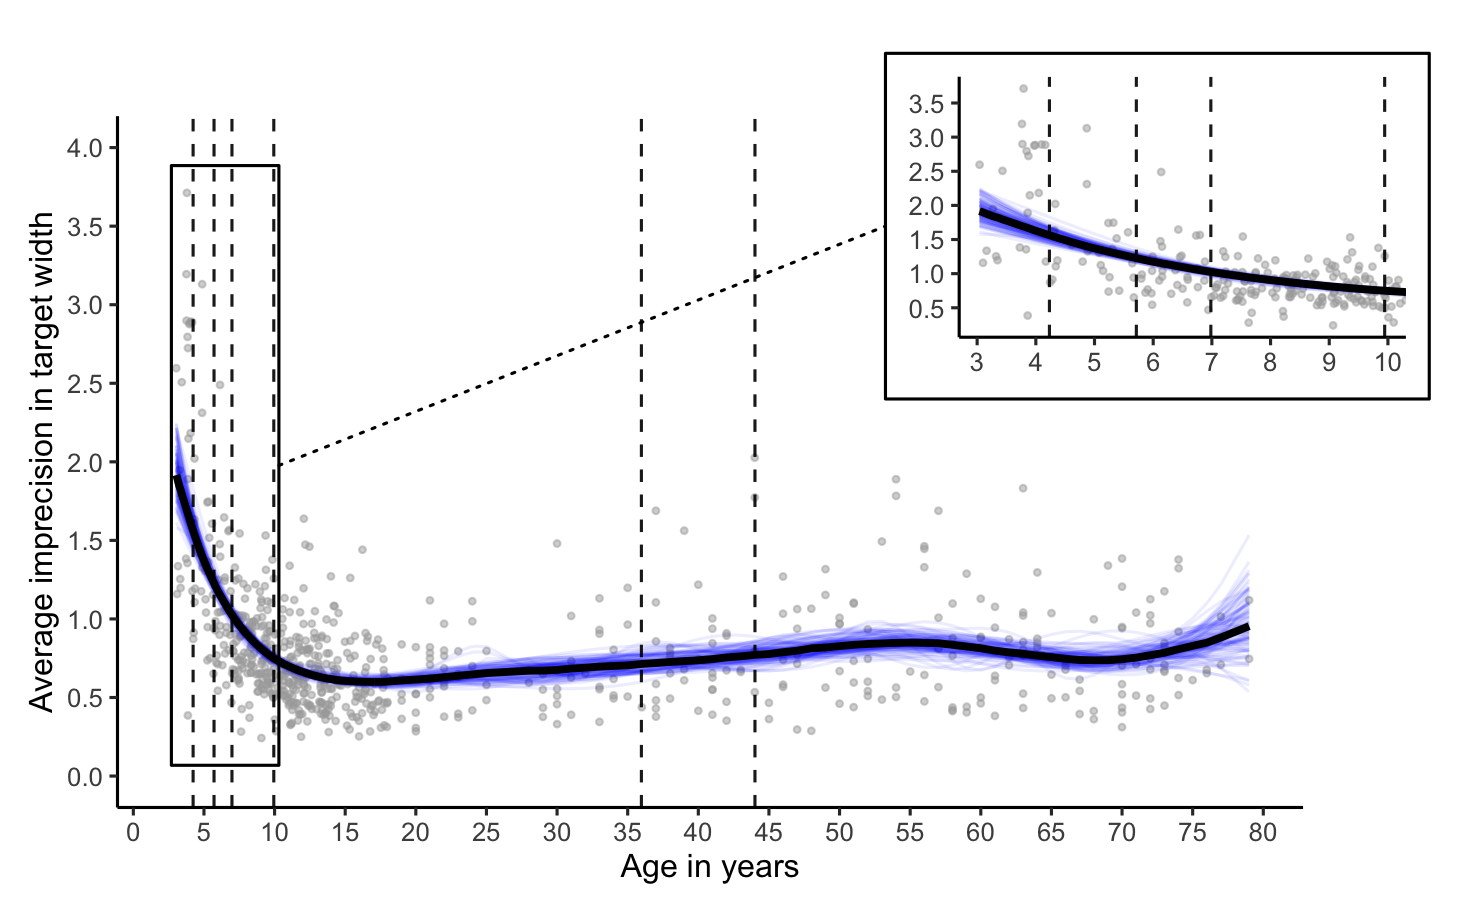
\includegraphics[width=1\linewidth]{../figures/lifespan_plot} 

}

\caption{\textbf{Developmental trajectory of gaze understanding across the lifespan}. Performance is measured as imprecision, i.e., the absolute distance between the target's center and the participant's click (averaged across trials). The unit of imprecision is counted in the width of the target, i.e., a participant with imprecision of 1 clicked on average one target width to the left or right of the true target center. Grey dots show the mean performance for each subject averaged across trials. Blue lines show 100 draws from the expectation of the posterior predictive distribution (i.e., conditional expectation) of the Gaussian Process model, with its mean predicted developmental trajectory as a solid black line. Vertical, black, dashed lines show the locations of the most prominent changes according to our Bayesian change point analysis.}\label{fig:fig1}
\end{figure}

High levels of variation pointed to individual differences in all age groups (overall imprecision mean = 0.81, sd = 0.82, range = {[}0 - 10.73{]}). For example, there were some children who were more accurate than the average adult.

In our model comparison, we found clear evidence for a non-linear development in gaze understanding across the lifespan. Compared against linear, quadratic, and cubic models, the Gaussian Process model showed the best model fit, demonstrated by the greatest model weight and smallest WAIC values. For the imprecision in gaze understanding, the standard deviation (\emph{b} = 1.52, 95\% CrI {[}0.25; 5.19{]}) and visual inspection indicated nonlinearity (see Figure \ref{fig:fig1}).

Going one step further, we investigated the most prominent change points in the data. The Bayesian change point analysis revealed 6 (with 23.49\% probability) major shifts in gaze understanding during the lifespan. The change points occurred at the following ages: 4.23 years (95\% CrI {[}4.13; 4.33{]}); 5.71 years (95\% CrI {[}5.38; 5.90{]}); 9.94 years (95\% CrI {[}8.66; 12.55{]}); 44.01 years (95\% CrI {[}40.37; 6.98 years (95\% CrI {[}6.64; 8.04{]}); 44.43{]}); and finally, at 35.97 years (95\% CrI {[}27.30; 39.69{]}). In other words: we found a very rapid initial improvement in early childhood, followed by a long period of minor, very slow change with slightly increasing levels of imprecision toward the eldest in our sample.

\hypertarget{discussion}{%
\subsection{Discussion}\label{discussion}}

We investigated the shape of change in gaze understanding across the lifespan. By applying the exact same task for the entire age range, we could directly compare gaze understanding in all ages. Therefore, we circumvented methodological challenges that often arise when trying to compare data across ages from qualitatively and quantitatively different study tasks.

We found a non-linear developmental trajectory in gaze understanding: Early in childhood, children quickly enhanced their level of proficiency. Performance peaked (i.e., imprecision was lowest) around early adulthood, while there was a minor decay in later adulthood. This is consistent with the view that we fine-tune our existing gaze understanding ability after the first emergence in early childhood. Furthermore, we observed individual differences in all age groups. While variation was highest in the three- and four-year-olds, it remained relatively stable across the lifespan.

Previous studies found that children start to follow gaze in the second half of their first year of life (Moll \& Tomasello, 2004). In our sample, three-year-olds were still rather imprecise in their gaze understanding ability. How can we explain this divergence? First of all, we used subtle eye movements as cues. Many existing studies let the agents move eye and head in parallel (Behne et al., 2005; Povinelli et al., 1997), therefore establishing a confound with more salient head movement. Relying exclusively on eye movements might be more difficult for children than presenting them with a combined eye and head orientation (Carpenter, Nagell, \& Tomasello, 1998). Furthermore, our study required participants to (1) precisely follow an agent's gaze, (2) interpret this as a cue, and then (3) make use of this cue to guide their own behavior (i.e., touching the screen at the cued location). We measured an active location choice instead of an attention orientation. It is conceivable that three-year-olds followed the agent's gaze but were still learning to translate this understanding into precise, active behavior.

Regarding the sample of elderly adults, we expect a sampling bias to be present (Bethlehem, 2010; Gosling, Vazire, Srivastava, \& John, 2004; Remillard, Mazor, Cutrona, Gurwitz, \& Tjia, 2014). First, certainly not all older people have a working high-speed Internet connection or are knowledgeable and trained in its use. Second, it takes a certain amount of independence and motivation to participate in \emph{Prolific} studies. The elderly who know how to participate in \emph{Prolific} studies might show greater cognitive fitness and flexibility compared to their offline counterparts. Therefore, a representative sample might show a greater age decline in gaze understanding compared to our reported sample. In addition, it is noteworthy that older people might be more likely to suffer from visual impairments. Even though we filtered participants to only include normal- to correct-to-normal vision, we cannot guarantee that our participants showed no symptoms of reduced vision.

\hypertarget{study-2-computational-cognitive-model}{%
\section{Study 2: Computational cognitive model}\label{study-2-computational-cognitive-model}}

Our lifespan study showed that gaze understanding develops throughout childhood, and variation between individuals appears in all age groups. The TANGO has previously been shown to reliably capture inter-individual differences in gaze understanding (Prein et al., 2023). The variation between participants is thus likely genuine and not due to random noise. Now, we aim to understand what explains the developmental change and the variation across participants on a process level. We present a theory of gaze understanding that explains how children process the available information (i.e., the agent's eyes) to make inferences about the agent's gaze and its attentional focus, which leads them to identify the target position. We formalize this inference process in a computational cognitive model.

Computational modeling frameworks allow researchers to establish mechanistic explanations of psychological phenomena (Grahek, Schaller, \& Tackett, 2021). As formal, mathematical accounts of the psychological process in question, they force researchers to accurately and comprehensively state all their underlying assumptions (Simmering, Triesch, Deák, \& Spencer, 2010). In addition, models can be used to simulate behavior and form testable predictions. The expected patterns can then, in turn, be compared to the empirically observed behavior.

We seek to explain how participants solved the TANGO. We designed a computational cognitive model that replicates a schematic representation of how participants make inferences in the task's context (i.e., model of the task and not the data). The fundamental assumption of this gaze model is that participants use all available gaze information to infer the target location.

Task design, data collection, and sample sizes were pre-registered: \url{https://osf.io/r3bhn}. The study design and procedure obtained ethical clearance by the MPG Ethics commission Munich, Germany, falling under a packaged ethics application (Appl. No.~2021\_45), and was approved by an internal ethics committee at the Max Planck Institute for Evolutionary Anthropology. The research adheres to the legal requirements of psychological research with children in Germany. Data were collected between May and August 2021.

\hypertarget{participants-1}{%
\subsection{Participants}\label{participants-1}}

The sample consisted of 60 children, including 20 three-year-olds (mean age = 3.47 years, SD = 0.34, range = 3.07 - 3.97, 11 girls), 20 four-year-olds (mean age = 4.61 years, SD = 0.26, range = 4.09 - 4.98, 10 girls), 20 five-year-olds (mean age = 5.66 years, SD = 0.24, range = 5.01 - 5.96, 12 girls). Data of children was collected in kindergartens located in Leipzig, Germany. The children within each kindergarten were recruited via an internal database, where each parent priorly consented to child development studies.

In addition, we included 50 adults from our Lifespan study (mean age = 31.92 years, SD = 12.15, range = 18 - 63, 36 female). Adults were recruited over \emph{Prolific} (Palan \& Schitter, 2018). Since developmental change was minimal in our adult sample (see Lifespan study) and the cognitive models were computationally heavy, we decided to only include the first 50 adults who had completed the study.

\hypertarget{procedure-1}{%
\subsection{Procedure}\label{procedure-1}}

We applied exactly the same procedure as in the first study, employing the continuous version of the TANGO (Prein et al., 2023). Children were tested in a quiet room in their kindergarten, while an experimenter guided the child through the study on a tablet. Adults participated online.

\hypertarget{computational-model}{%
\subsection{Computational model}\label{computational-model}}

Our model quantifies a participant's cognitive ability to follow gaze by inverting a probabilistic process that generates the participant's clicks from observing the eyes of the agent. It is formally defined as:

\begin{equation}
    P(\theta | x_c, \alpha_l, \alpha_r) \propto P(x_c | \alpha_l, \alpha_r, \theta)P(\theta)
\end{equation}

where \(\theta\) is an individual's cognitive ability to locate the focus of the agent's attention, \(x_c\) is the coordinate the participant clicked, and \(\alpha_l\) and \(\alpha_r\) are the pupil angles for the left and right eye, respectively. The pupil angle \(\alpha\) is defined as the angle between a line connecting the center of the eye to the pupil and a line extended vertically downward from the center of the eye (see \ref{fig:fig2}A).\footnote{This model mirrors the logic of the TANGO programming code. In the online experiment, we read out the center point coordinates of the target and the agent's eyeball (i.e., the SVG coordinates). We then calculate a line between these two points: this is our gaze vector (acting in the functionally same way as a pupil angle). Now, knowing the eyeball radius, we calculate the point of intersection at which the gaze vector meets the eyeball boundary. Finally, the agent's pupil moves from the center of the eyeball along the gaze vector to the intersection point. This way, the agent is animated to ``look at'' the target. In the gaze model, we assume participants go through these steps in reverse order.}

Based on our verbal task instructions, we assume that participants (1) expect the agent's looks to be directed at the target, and (2) to click on the coordinate they estimate the agent to look at. Consequently, we do not assume that participants' clicks are noisy in any way but that they click on the screen location where they genuinely think the target is (and that the agent is looking at). However, the true eye angles (\(\alpha_l\) and \(\alpha_r\)) cannot be directly observed. These have to be estimated based on the position of the pupils within the eyes, resulting in approximate values (\(\hat{\alpha_l}\) and \(\hat{\alpha_r}\)). We presume this estimation to be a noisy process. Thus, the development of the cognitive ability to follow gaze corresponds to a reduction in the magnitude of the noise in the estimates (i.e., an increased certainty about the pupil angles).

Any clicked value of \(x_c\) implies a ``matched pair'' of the estimated pupil angles \(\hat{\alpha_l}\) and \(\hat{\alpha_r}\), with the property that lines extended along those two angles meet at the precise location of the target. As a consequence, we can rewrite the likelihood function of the model above:

\begin{equation}
P(x_c | \alpha_l, \alpha_r, \theta) \propto P(\hat{\alpha_l}, \hat{\alpha_r} | \alpha_l, \alpha_r, \theta) P(x_c)
\end{equation}

The second term of the right-hand side equation above, \(P(x_c)\), is a prior over potential target locations, which we assume to be skewed towards the screen center: We anticipate that participants have an a priori expectation that the target will land close to the middle, partly because the target was last visible in the screen center before disappearing behind the hedge, and because the agent is located centrally on the screen. We estimate the strength of this center bias (i.e., the standard deviation of a Normal distribution around the center of the screen) based on the data.

We estimated \(P(x_c)\) as a deviation from a hyper parameter: \(P(x_c)_i \sim \mathcal{N}(960,\sigma^{P(x_c)_j})\). Please note that µ = 960 specifies the center of the screen. To allow developmental effects in this center bias, we defined \(P(x_c)_j\) via a linear regression as a function of the participant's age (\(age_i\)): \(P(x_c)_j = \beta_0^{P(x_c)} + age_i \cdot \beta_1^{P(x_c)}\). Therefore, the participant-specific value for \(P(x_c)\) was constrained by the performance in the TANGO and the participant's age.

The main inferential task for the participant lies in estimating the pupil angles, i.e., sampling from the first term of the right-hand side equation above, \(P(\hat{\alpha_l}, \hat{\alpha_r} | \alpha_l, \alpha_r, \theta)\). For this, we assume that the pair of estimated pupil angles are sampled from a probability distribution which is the product of two Normal distributions of equal variance \(\sigma_v\) centered on the true pupil angles:

\begin{equation}
P(\hat{\alpha_l}, \hat{\alpha_r} | \alpha_l, \alpha_r, \theta) \propto \phi(\hat{\alpha}_l ; \alpha_l, \sigma_v)\phi(\hat{\alpha}_r ; \alpha_r, \sigma_v),
\end{equation}

Broadly summarizing: Participants are assumed to observe the pupil locations and the center of the agent's eyes. Connecting these two point estimates as a line yields the unique vector that extends from the center of the agent's eyeball through the center of the pupil to the attentional focal point. Taking the angle between this vector and a line pointing vertically to the ground yields the pupil angle. Participants are assumed to sample from Normal distributions centered around the true pupil angle. They are assumed to do this independently for the left and right eye and then integrate the information to estimate the target's location.

As \(\sigma_v\) determines the level of accuracy with which the participant estimates the pupil angles, it is the component that defines \(\theta\). When \(\sigma_v\) is very small (i.e., the distribution around the pupil angle is narrow), clicks far away from the target are unlikely, as these would require estimated pupil angles very different from the true pupil angles.~When \(\sigma_v\) is very large (i.e., the distribution around the pupil angle is wide), almost any pupil angles may be sampled, corresponding to a roughly uniform distribution over click coordinates. We expect \(\sigma_v\) to vary between individuals. Consequently, individuals differ in the level of precision with which they can locate the target based on observing the agent's eyes.

The shape of the \(P(x_c | \alpha_l, \alpha_r, \theta)\) distribution leads to an interesting, testable group-level prediction. As the pupil location varies, a fixed amount of uncertainty around the pupil angle corresponds to a varying degree of uncertainty in the estimated target location. When the agent directs their gaze toward the very left or right side, the distribution around the pupil angle from which participants sample is comparatively wider than when the agent gazes centrally to the ground in front of them (see \ref{fig:fig2}D). For illustrative purposes, imagine a similar phenomenon: pointing a torch light to a flat surface on the ground. When one points the light cone directly at the surface, the light beam is concentrated in a clearly defined, small, symmetric area. When one points the light cone further away from oneself (shining at an angle), the light from one half of the cone must travel further to reach the surface than the light from the other half, resulting in an asymmetric light pattern. As the angle increases, the light is spread over a wider area, and the surface is illuminated less evenly. Consequently, for the same \(\sigma_v\), the further out a target coordinate lies, the wider and less symmetric the distribution. This increases both the variance and the bias in a participant's estimate of the agent's attentional focus, resulting in a decreased performance in the task. As \(\sigma_v\) decreases and the cone narrows, the extent to which performance varies at different angles decreases. Therefore, our gaze model predicts that our trials vary in difficulty: participants should be more imprecise in locating the target the further out it lands.\footnote{In our screen-based study, this effect should decrease again towards the most outward sides. Since the computer screen has a natural border, trials in which the target lands furthest out to the left/right become slightly easier again. In these cases, the uncertainty about the pupil angle faces practically only the inner side (facing the center) of the screen, since the natural border of the screen limits where participants can click. In another adult sample with more trials, we could recover this pattern. For further elaboration, see Supplements.} If our data matches the pattern of this model prediction, this can act as evidence for the gaze model. Therefore, our gaze model provides a quantitative theory of gaze understanding with testable model predictions.

\hypertarget{analysis-1}{%
\subsection{Analysis}\label{analysis-1}}

Our goal was to describe the inferential process of gaze understanding. We quantified how well our gaze model explained the gaze understanding process by comparing it to two alternative models that make different assumptions of which information participants use and where they consequently click to locate the target. Our modeling framework consisted of three mutually exclusive models: (1) a gaze model, (2) a random guessing model, and (3) a center bias model. We gauged which model can best explain our data by conducting model comparisons. All cognitive models were implemented in WebPPL (Goodman \& Stuhlmüller, 2014).

To gauge the plausibility of our gaze model, we implemented two models that represent alternatives about how participants solve the TANGO. Participants who were overall very imprecise in locating the target might be less likely to use the agent's gaze as a cue at all. The alternative models, therefore, do not assume that participants made use of the gaze cue. The first alternative model assumed participants were randomly guessing. This was implemented as sampling from a uniform distribution over all possible coordinates, \(\mathcal{U}(0, 1920)\). The second alternative model assumed the participants always wanted to click at the screen center: Participants could be drawn toward the screen center since the agent and the starting point of the balloon were located there. This was implemented as sampling from a Normal distribution, \(\mathcal{N}(960, 160^2)\), with the the center of the screen as the mean, and one target width as the standard deviation.

Our three proposed models made different predictions about how participants' clicks would be distributed for different target locations. We visualized and evaluated these differences using correlations between the model predictions and the data. For this, we converted the models' posterior distributions for each participant into a single value by taking the mode (and 95\% highest density interval--HDI). Furthermore, we evaluated these probabilistic models based on the marginal likelihood of the data under each model. The pairwise ratio of marginal likelihoods for two models is also known as the Bayes Factor. This factor quantifies the quality of a model's predictions by averaging over the possible values of the model's parameters weighted by the prior probabilities of those parameter values. It can be used to estimate how much more likely the data under one model are compared to the other. Bayes Factors implicitly consider model complexity (i.e., Bayesian Occam's razor): models with more parameters often have a broader prior distribution over parameters, which might weaken potential gains in predictive accuracy. Details on models, including code to run the models, information about priors for parameter estimation, and Markov chain Monte Carlo settings, can be found in the associated online repository.

\hypertarget{todo-add-more-infos-on-priors-parameters}{%
\subsection{{[}TODO: add more infos on priors \& parameters{]}}\label{todo-add-more-infos-on-priors-parameters}}

\hypertarget{results-1}{%
\subsection{Results}\label{results-1}}

We found clear support for our gaze model, both in children as well as adults. The Bayes Factors we computed via the marginal likelihood of the data strongly favored our gaze model compared to the center bias model (\(logBF_{10}\) = 1,015.33) and the random guessing model (\(logBF_{10}\) = 388.98).
When correlating the observed data across all target positions with the predictions of the three models, we found a high similarity for the gaze model: \emph{r} = 0.95, 95\%CI {[}0.90, 0.98{]}, while the correlations with the alternative models were substantially smaller (center bias model: \emph{r} = 0.77, 95\%CI {[}0.57, 0.89{]}; random guessing model: \emph{r} = 0.78, 95\%CI {[}0.58, 0.89{]}). The developmental trajectory of the estimated gaze model parameter also correlated highly with the observed data: \emph{r} = 0.95, 95\%CI {[}0.92, 0.97{]}. The age effects in Study 2 largely replicated those of Study 1.



\begin{figure}

{\centering 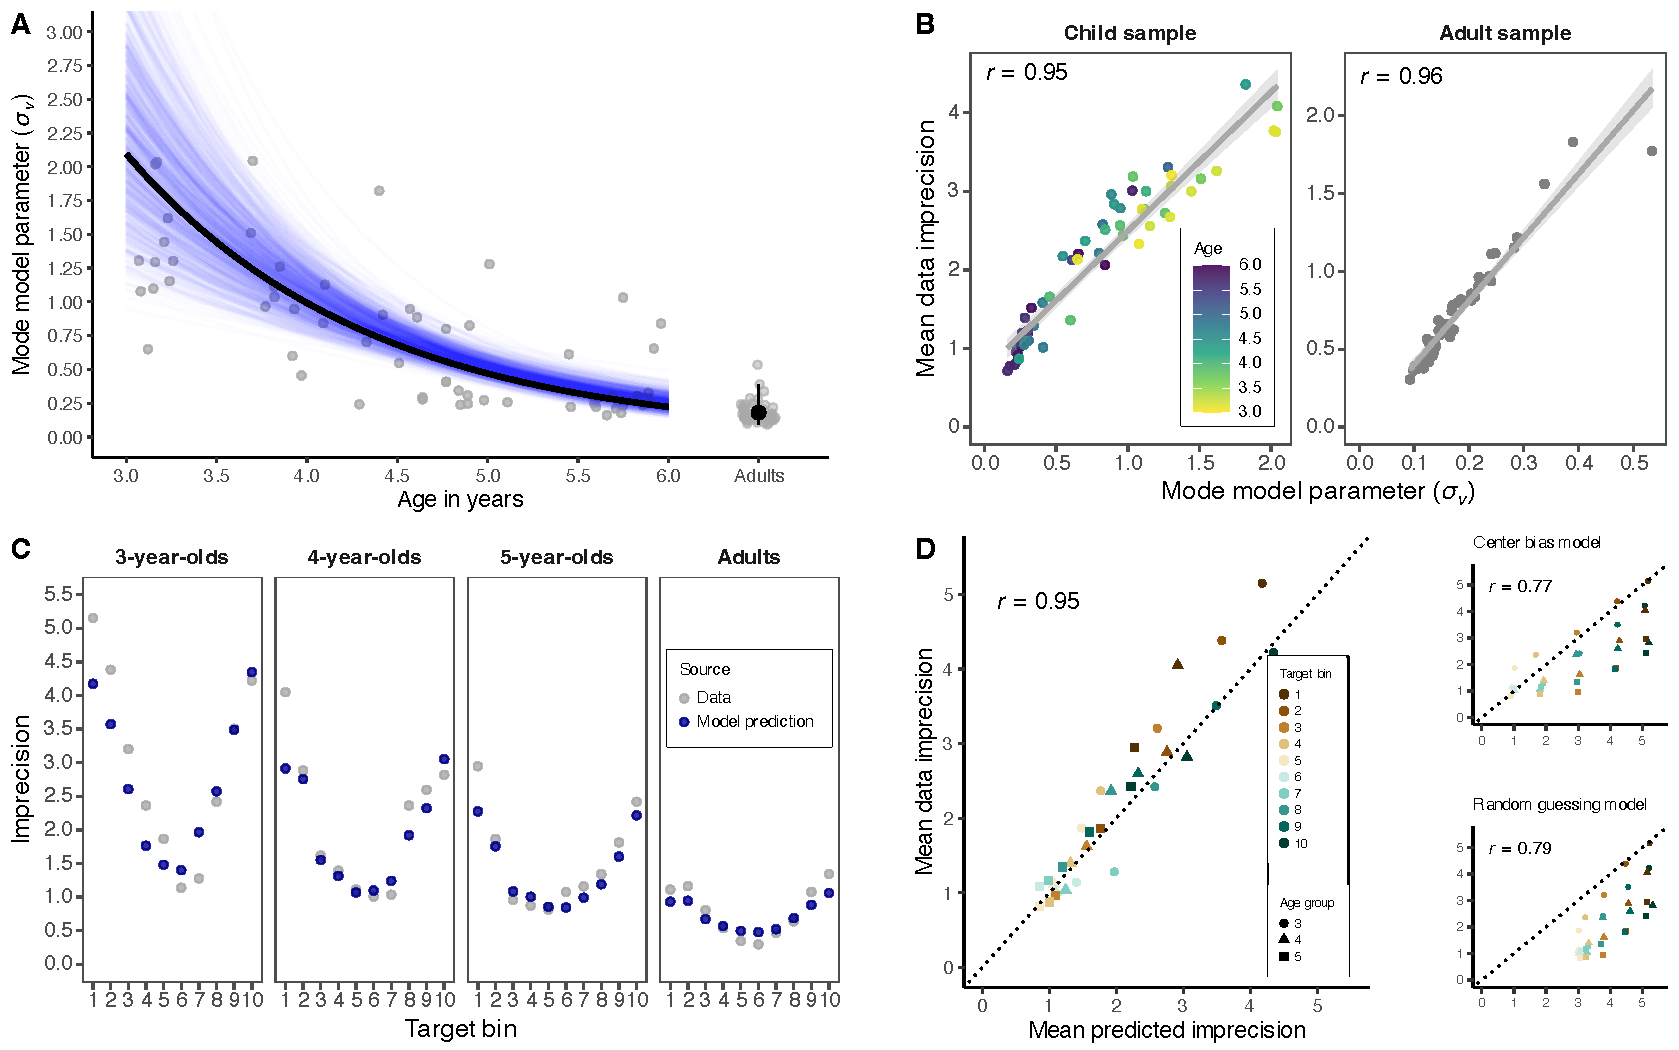
\includegraphics[width=1\linewidth]{../figures/gazemodel_plot} 

}

\caption{\textbf{Gaze model} (A) Visualization of the gaze model. Participants are assumed to observe the pupil location and estimate the center of the agent's eye. Connecting these two point estimates as a line yields the unique vector that extends from the center of the agent's eyeball through the center of the pupil to the attentional focal point. Taking the angle between this vector and a line pointing vertically to the ground (black dashed line) yields the pupil angle (\(\alpha\)). Participants are assumed to sample (grey lines) from Normal distributions (blue line) centered around the true pupil angle (\(\alpha\)). The variance around the Normal distribution (\(\sigma_v\)) is centered on the true pupil angle and expected to vary between participants. (B) Developmental trajectory of the estimated model parameter. Grey dots show individual level parameter values. The black line shows the maximum a posteriori (MAP) estimate; blue lines show 1000 draws from it. (C) Correlation between estimated mode of the model parameter and data mean per individual, color-coded by age. The grey regression line with 95\% CI shows smooth conditional mean based on a linear model, with \emph{Pearson}'s correlation coefficient \emph{r}. (D) Geometrical features of the gaze model. As the pupil location varies, a fixed amount of uncertainty around the pupil angle corresponds to a varying degree of uncertainty in the estimated target location. Top: Agent gazes centrally to the ground. Bottom: Agent gazes toward the side. The distribution around the pupil angle from which participants sample is wider compared to when the agent gazes centrally. The blue line on the ground shows the added level of uncertainty in the estimated target position for the target location further outward. (E) Pattern recovery. Imprecision in target width for each target bin by age group. Model predictions in blue; data in grey. (F) Correlation between the observed data and the predictions of the three models by target position (across age and individuals).}\label{fig:fig2}
\end{figure}

\hypertarget{discussion-1}{%
\subsection{Discussion}\label{discussion-1}}

Our findings from Study 1 showed individual differences and a developmental change in gaze understanding across the lifespan To answer what develops with age and how participants differ from one another, we presented a formal cognitive model of gaze understanding. Participants are modeled to observe all available gaze information, integrate it from both the agent's eyes, and consequently arrive at the attentional focus of the agent: the target location. We assume the basic process of gaze understanding to be the same across the lifespan, though individuals become increasingly precise with age. By conducting model comparisons, we could rule out that participants' responses can be explained by random guessing or a center bias.

In addition, we observed differences in performance depending on where the agent looks. The observed data showed that precision levels dropped as the agent's gaze moved further away from the center. Our gaze model predictions recovered this ``signature pattern'' in the data. Future research could use this signature in the data as evidence of whether diverse communities employ the same inferential mechanism to solve the task, speaking for a shared cognitive architecture.

Interestingly, the U-shaped pattern in the TANGO task can be conceptually compared to the result patterns of Michelon and Zacks (2006): in their Level 1 perspective-taking visibility task, an increased distance between the agent and the target decreased performance (i.e., reaction times). Additionally, targets closer to the midline were more easily traced than ones further away from the agent. The authors concluded that visual acuity is generally higher for locations on the vertical axis than for those on diagonal axes (cf.~``oblique effect''; (Appelle, 1972; Heeley, Buchanan-Smith, Cromwell, \& Wright, 1997; Mikellidou, Cicchini, Thompson, \& Burr, 2015)). Not only is our finding of increased imprecision for greater pupil angles (i.e., trials in which the target lands further out) consistent with this finding, but our gaze model poses a viable explanation for this effect.

A limitation of our model is that we cannot disentangle how much of the participants' uncertainty comes from a noisy estimate of the agent's attentional focus and how much is due to imprecise clicking (e.g., wanting to click somewhere but experiencing motor issues at aiming, adding random noise to the click).

A critical feature of our model is that it assumes gaze understanding to rely on vector estimation. In other words, subjects are modeled to calculate pupil angles which serve as gaze vectors to point to the attentional focus point of an agent. Even though this vector estimation component is a rather physical, geometrical calculation, it still happens in a social context. In the first place, one must interpret the agent's eyes as a relevant social stimulus. Therefore, our computational model describes gaze understanding as a particular form of vector estimation in a social context.

\hypertarget{study-3-components-of-gaze-understanding}{%
\section{Study 3: Components of gaze understanding}\label{study-3-components-of-gaze-understanding}}

We previously presented a computational cognitive model of gaze understanding. Our model relies on the perhaps unexpected assumption that vector estimation is a crucial component of gaze understanding. In model comparisons, we found overwhelming support for this model in children and adults. Now, we wanted to test this assumption experimentally. We were interested in the degree to which vector estimation is a part of gaze understanding. Additionally, we investigated whether there is more to gaze understanding than the physical vector estimation component. To answer this question, we assessed the relationship between gaze understanding and other social-cognitive abilities. We reasoned that gaze understanding is integral to social interaction, which is most likely learned in the social world. The positive link between TANGO and family-level variables like number of siblings (Prein et al., 2023) underlines this. Therefore, it seems reasonable to expect correlations between gaze understanding and other social-cognitive abilities.

First, we aimed to experimentally isolate the vector estimation component of the TANGO. We designed a new non-social vector estimation task that shared all crucial design features of the TANGO. Second, we assessed children's social-cognitive abilities by administering a Theory of Mind (TOM) task battery, comprising four tasks from the ToM scale by Wellman and Liu (Wellman \& Liu, 2004) and two additional perspective-taking tasks (Flavell, Everett, Croft, \& Flavell, 1981; Flavell, Flavell, Green, \& Wilcox, 1981).

We aimed to assess whether there are exclusively task-specific processes at hand or whether gaze understanding recruits a general social-cognitive ability that is shared among other social-cognitive tasks. We reasoned that the TANGO shares task demands with the non-social vector estimation task while it shares its social context with the ToM tasks. This way, we aimed to disentangle what components comprise gaze understanding.

Task design, data collection, and sample sizes were pre-registered: \url{https://osf.io/xsqkt}. Data were collected between February and March 2023.

\hypertarget{participants-2}{%
\subsection{Participants}\label{participants-2}}

Testing took place in kindergartens in Leipzig, Germany. The sample consisted of 102 children (mean age = 4.54 years, SD = 0.31, range = 3.99 - 5.03, 54 girls). Information on individual socio-economic status was not formally recorded.

\hypertarget{procedure-2}{%
\subsection{Procedure}\label{procedure-2}}

Children were tested in a quiet room in their kindergarten. An experimenter guided the child through the study. Since our research questions related to individual differences and we wanted maximum control of extraneous participant variables, we employed a within-subjects study design. All participants performed the following tasks in a fixed order: (1) non-social vector estimation task, (2) ToM task battery, (3) TANGO. Several reasons motivated this decision. First, we decided on a fixed order to be able to compare participants' performance straight-forwardly with each other. Second, to increase participant engagement and decrease fatigue or fuzziness, we switched from a tablet task to tasks with personal interaction back to a tablet task. Third, we showed the non-social vector estimation task before the TANGO so that participants would not be biased to interpret the presented stimuli as ``eye- /''agent-like''.

\hypertarget{non-social-vector-estimation}{%
\subsubsection{Non-social vector estimation}\label{non-social-vector-estimation}}

Modeling the setup and structure of the previously applied TANGO, we designed a non-social vector estimation task. This task was also presented as a web application on a tablet and made use of the concept of magnetism. The setup looked as follows. On the upper part of the screen, there was a tube with a gearwheel located in a circular window. On the floor, there was a magnet. The magnet then got switched on (making a cartoon-like sound), whereupon the gearwheel moved towards the magnet. The gearwheel moved in a way that its center aligned with the center of the magnet, while staying inside the circular window. Participants were then asked to locate the magnet. Access to the magnet's true location was manipulated by a wooden wall: participants either had full, partial, or no visual access to the true magnet location. When no information about the magnet location was accessible, participants were expected to use the gearwheel inside the window as a non-social cue to locate the magnet.

As in the TANGO, there were three different trial types depending on the visual access to the true magnet location. In full visual access trials, the magnet's location was presented without impediment (i.e., no wooden wall). In partial visual access trials, the wooden wall was moved in front of the target after the magnet's location had already been visible. In test trials, participants had no visual access to the magnet's location because the wall covered the magnet from the beginning of the trial.

Children received 19 trials with one full visual access trial, two partial visual access trials, and 16 test trials. The first trial of each type comprised a voice-over description of the presented events. We conducted our analysis with 15 test trials (excluding the voice-over trial). The outcome variable was imprecision, defined as the absolute difference between the magnet's x coordinate and the x coordinate of the participant's click. Magnet coordinates were generated as follows. The full width of the screen was divided into ten bins. Each bin occurred equally often, while the same bin could occur in two consecutive trials. Exact coordinates within each bin were randomly generated.

\hypertarget{tom-task-battery}{%
\subsubsection{ToM task battery}\label{tom-task-battery}}

We administered four tasks from the Wellman and Liu (2004) ToM scale. We excluded three tasks: the Diverse Desires task in order to avoid ceiling effects; and both tasks involving emotions (Belief Emotion and Real-Apparent Emotion), as we aimed at assessing the ``cold, cognitive'' (as compared to the ``emotional'') aspects of social cognition. Instead, we added two perspective-taking level-2 tasks (Flavell, Everett, et al., 1981; Flavell, Flavell, et al., 1981). We added the perspective-taking tasks (1) with the aim of increasing the variablility we can capture between individuals, and (2) since we hypothesized that perspective-taking would rely on similar mechanisms than gaze understanding. The dependent variable was the aggregate score of all solved ToM tasks (see Supplements for further detail). Additionally, we investigated if gaze understanding was more strongly associated with the two perspective-taking tasks compared to the other ToM tasks, as perspective-taking seems most closely theoretically related to gaze understanding (i.e., in both cases the participant is asked to judge another person's point of view).

\hypertarget{gaze-understanding}{%
\subsubsection{Gaze understanding}\label{gaze-understanding}}

As in the two previously reported studies, we presented children with the continuous version of the TANGO (Prein et al., 2023). To accentuate the social aspect of the TANGO, we exchanged the animal agents (used in the previous two studies) with human faces, which were modeled after the local population in appearance (already created for another project on cross-cultural similarities in gaze understanding (\url{https://osf.io/tdsvc})). This further highlighted the contrast (i.e., social vs.~non-social context) to the non-social vector estimation task.\footnote{In an exploratory analysis, we compared children's imprecision levels in the TANGO task with animal vs.~human agents. Based on a GLMM analysis, we conclude that there was no evidence of a stable effect of stimulus choice (human vs.~animal). See Supplements for further detail.}

\hypertarget{analysis-2}{%
\subsection{Analysis}\label{analysis-2}}

By design, both the TANGO as well as the non-social vector estimation task involve vector estimation. On the basis of the results from our computational cognitive model, we expected that children's performance in both tasks correlate with each other. For each of these two tasks, we calculated the mean level of imprecision for each subject. We then correlated these two scores using \emph{Pearson's} correlation coefficients.

Regarding the relationship between the two vector estimation tasks and the ToM measures, we could imagine two possible scenarios: (A) If gaze understanding recruits a general social-cognitive ability beyond vector estimation, we expected that gaze understanding and ToM measures would correlate more strongly with each other than non-social vector estimation and ToM measures. (B) If gaze understanding relies purely on task-specific processes, then the correlation between gaze understanding and ToM measures would be comparable to the correlation between non-social vector estimation and the ToM measures. For the association between the aggregate ToM scores and the gaze understanding / non-social vector estimation tasks, we used \emph{Spearman's} rank correlation coefficients.

We compared the correlation between gaze understanding and ToM measures and the correlation between non-social vector estimation and ToM measures by using the Williams' test from the function \texttt{cocor.dep.groups.overlap} (designed for two dependent overlapping correlations) from the package \texttt{cocor} (Diedenhofen \& Musch, 2015).

Furthermore, to estimate which components best explain the gaze understanding score, we conducted a model comparison with GLMMs predicting the mean imprecision in gaze understanding by age, imprecision in non-social vector estimation, the ToM aggregate score, or the aggregate of the two perspective-taking tasks (subset of ToM battery; example of model notation in \texttt{R:\ tango\_mean\ tilde\ age\_centered\ +\ magnet\_scaled\ +\ perspective\_scaled}). We wanted to assess whether the ToM aggregate score or the singled-out perspective-taking score added additional explanatory value when predicting the gaze understanding score. The outcome variable was modeled by a lognormal distribution.

\hypertarget{results-2}{%
\subsection{Results}\label{results-2}}

As expected, we found that gaze understanding as a social vector estimation task correlated with the non-social vector estimation task, \emph{r} = 0.38, 95\%CI {[}0.20, 0.53{]}. Importantly, however, the two vector estimation tasks were not redundant: only a part of the variance in gaze understanding could be explained by non-social vector estimation.

Gaze understanding and perspective-taking showed a \emph{Spearman} correlation coefficient of \(\rho\) = -0.29, 95\%CI {[}-0.46, -0.10{]}, while non-social vector estimation and perspective-taking did not correlate, \(\rho\) = -0.09, 95\%CI {[}-0.28, 0.10{]}. According to the Williams' test, these two correlations did not differ significantly from each other, \emph{t}(99) = -1.86, \emph{p} = 0.07.

Our model comparison revealed that gaze understanding was best predicted by a model including non-social vector estimation (\(\beta\) = 0.14, 95\% CrI {[}0.06; 0.21{]}) and perspective-taking (\(\beta\) = -0.10; 95\% CrI {[}-0.17, -0.03{]}), even when controlling for age (\(\beta\) = -0.14, 95\% CrI {[}-0.38, 0.10{]}). See Supplements for further detail of the model comparison.

Taken together, this shows that the TANGO recruited social-cognitive abilities beyond vector estimation. Evidently, it shared some of its variance with other level 2 perspective-taking tasks, while the overall ToM aggregate score did not add explanatory power.



\begin{figure}

{\centering 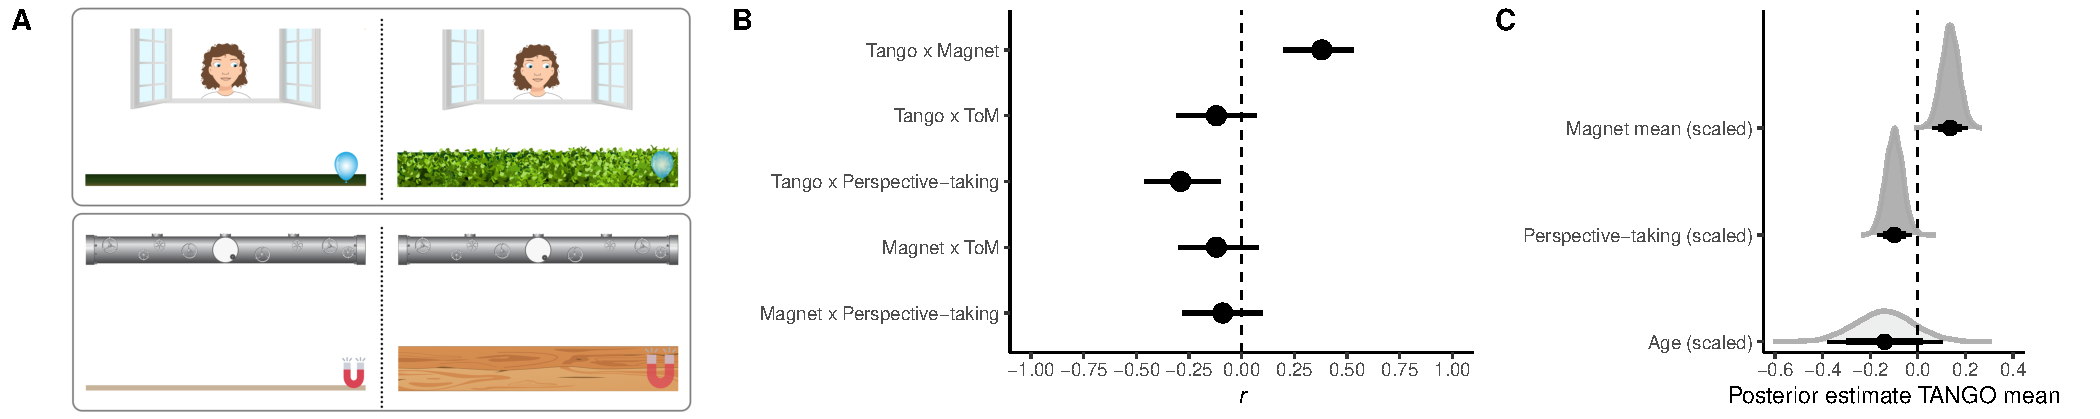
\includegraphics[width=1\linewidth]{../figures/magnet_plot} 

}

\caption{\textbf{Components of gaze understanding.} (A) Study procedures. Top: TANGO (i.e., gaze understanding; social vector estimation). Bottom: Magnet (i.e., non-social vector estimation). Left hand side show screenshots of familiarization phase; right hand side show screenshots of the test phase. (B) Correlations between gaze understanding, physical vector estimation, ToM, and perspective-taking. Dots show the correlation coefficients, while error bars represent 95\% CIs. (C) Influence of age, perspective-taking and physical vector estimation on gaze understanding. The graph shows the posterior distributions for the respective predictor. Black dots represent means, thicker black lines 80\% CrI and thinner black lines 95\% CrI.}\label{fig:fig3}
\end{figure}

\hypertarget{discussion-2}{%
\subsection{Discussion}\label{discussion-2}}

By carefully isolating physical vector estimation experimentally, we could show that gaze understanding does indeed, to a certain degree, rely on this component. This is in line with our computational cognitive framework that assumes vector calculations on a process-level. However, physical vector estimation alone did not suffice to explain gaze understanding. In addition, perspective-taking proved to be a relevant social-cognitive ability when predicting the performance in the TANGO.

Both the TANGO and the two applied perspective-taking tasks can be seen as instances of \emph{visuospatial perspective-taking.} According to Surtees, Apperly, and Samson (2013), perspective-taking tasks involve three components: (1) a Self (i.e., the perspective-taker), (2) the Other (i.e., a target perspective that gets judged), and (3) an Object (which is taken into perspective).
One can roughly categorize them into two groups.

Level 1 perspective-taking, also termed visual accessibility judgment, is concerned with the visibility of objects from a particular viewpoint. In these tasks, participants judge whether an object is located before or behind an agent and if this agent can see it (Surtees et al., 2013). Usually, participants can solve these tasks independently from another's agent frame of reference and do not need to apply mental rotation (not matching the ``mentalizing criterion''; (Quesque \& Rossetti, 2020)).

Level 2 perspective-taking, however, does rely on a mental transformation of oneself into the space of another agent. In these tasks, participants judge how (visually or conceptually) the world looks like for another person or whether an object is to their right or left. This presumably entails a simulative transformation of one's own body schema (Erle \& Topolinski, 2017). Additionally, participants must understand that different viewpoints lead to different perspectives (Flavell, Everett, et al., 1981): two agents can see the same object ``in different, incompatible, fine-grained ways'' (Rakoczy, 2022).

In short, Level 1 perspective-taking addresses \emph{what} an agent can see, while Level 2 perspective-taking addresses \emph{how or where} they see it (Moll \& Tomasello, 2006). The TANGO falls into the first category - however, in contrast to existing research, on a continuous scale. The two perspective-taking tasks we administered within the ToM scale fall into the second category.

What drives the connection between the TANGO and the two other perspective-taking tasks? Both tasks tap into the ability to judge what another person sees. In the TANGO, participants must assume that another agent perceives and looks at the target in order to locate it. The here-used perspective-taking tasks add a layer by asking how one's perspective differs from another person's and how exactly the other person sees an object. In an intriguing series of experiments, Michelon and Zacks (2006) assessed the different processes that participants used to master Level 1 (visibility of objects) and Level 2 (object's location relative to another agent) perspective-taking tasks. Their results suggest that participants rely on line-of-sight tracing in the former case and perspective transformation in the latter case. According to (Michelon \& Zacks, 2006), \textbf{line-of-sight tracing} presumably consists of (1) locating the avatar, (2) locating the target, and (3) drawing a line from the agent to the target. Note how our gaze model in Study 2 shares the underlying idea of connecting points in space via a line.

Perspective transformation presumably adds complexity and consists of: ``(1) locate the avatar in an egocentric space, (2) perform a perspective transformation so that one's imagined position matches the position of the avatar, (3) locate the target object in the transformed spatial representation of the scene, and (4) read off the coordinates of the object'' (Michelon \& Zacks, 2006). Therefore, the processes to solve Level 1 perspective-taking tasks might be computationally lighter since there is no need to adapt the other person's reference frame. Still, the assumed processes overlap, which could explain the correlation between the TANGO and the administered perspective-taking tasks.

Why doesn't gaze understanding correlate with the other ToM tasks? While ToM tasks and the TANGO share the social context, the cognitive processes needed to solve each task might vary. As Rakoczy (2022) reflected, perception-goal psychology (which includes gaze understanding) comprises understanding that others see different objects or pursue different goals. However, this ability does not necessarily entail understanding more complex meta-representational aspects; for example, understanding that mental states can be mutually incompatible, false, or involve fine-grained aspectual information.

Surtees et al. (2013) further differentiate between visual and perspective-taking. While the former helps to judge if and how an agent sees an object, the latter involves judging the relative spatial locations of an agent and the object. Spatial perspective-taking can work without mental states and can, therefore, be applied to non-agentive objects with a front (Surtees et al., 2013). Interestingly, computing a line of sight does not demand the presence of another agent (Michelon \& Zacks, 2006). This could explain how our participants solved the non-social vector estimation task.

In previous work, we could establish that the TANGO is suited as an individual differences measure (Prein et al., 2023). Capturing meaningful variability in performance is a crucial task feature when we are interested in revealing the relationship between different cognitive abilities. Importantly, the tasks we used to measure ToM abilities were not designed to capture individual differences: they relied on an aggregate score of few dichotomous trials. These sum scores contan measurement errors and can only capture limited variance, which may obscure potential correlations. However, since these tasks are the gold standard in the social-cognitive literature and continuous measures with satisfying psychometric properties are, to the best of our knowledge, still scarce, we nonetheless relied on them in this study. It seems noteworthy to point out that lower correlations between ToM abilities and gaze understanding could be grounded in the design features of the applied ToM tasks. We already stated this concern in the Pre-registration (\url{https://osf.io/xsqkt}).

If the reliability of a certain task is known, one can estimate the ``true'' correlation between the latent constructs by applying an attenuation formula or structural equation models (Metsämuuronen, 2022; Trafimow, 2016, 2016). Adjusting for the measurement error would most likely increase the underlying correlation. While we can estimate the split-half reliability (stratified by target position) for the TANGO and the non-social vector estimation task (for example, see {[}prein2023tango{]}), we do not have reliability estimates of the ToM measures. Therefore, applying said approaches is unfortunately not feasible to compare correlations between all our applied measures. This, in turn, underlines the importance of the psychometric properties of a task and the reporting of such.

The development of new measures to capture individual differences in social-cognitive abilities like false-belief understanding seems desirable and essential to move this line of research further.

\hypertarget{general-discussion}{%
\section{General discussion}\label{general-discussion}}

In this paper, we have illuminated the developmental trajectory of gaze understanding and the cognitive processes behind it. Study 1 focussed on how gaze understanding changes with age. We found that individual differences exist throughout the lifespan. There is a steep learning curve in the preschool years in which children become more and more precise in locating the attentional focus of an agent. During teenage years and early adulthood, participants reach their peak performance. Precision levels then stay comparably stable, with a minor decay toward older adulthood. In Study 2, we proposed a computational cognitive model that describes gaze understanding at a process level. Our gaze model estimates reliable individual parameter values and could recover signature patterns in the data. It outperformed two alternative models, which assumed participants solved the task via a center bias or random guessing. Study 3 made use of the case that the TANGO is a reliable individual differences measure to further investigate potential components of gaze understanding. One fundamental assumption of our computational cognitive model is that gaze understanding relies on a vector estimation process. We experimentally isolated this component by carefully designing a non-social, physical vector estimation task. Furthermore, we assessed the relationship between gaze understanding and traditional ToM tasks. We found that gaze understanding does, indeed, share a substantial part of its variance with the non-social counterpart of physical vector estimation. In addition, perspective-taking correlated with gaze understanding, whereas the other ToM measures (focussing on diverse desires, knowledge access, and false beliefs) did not.

The developmental trajectory seen in Study 1 shows how abilities that emerge in infancy can continue to develop throughout childhood. While previous research established that one-year-olds can orient their visual attention toward one out of two objects, this is not the end point of development. By studying gaze understanding on a continuum, we could move beyond the pure existence of gaze understanding and assess how precisely children locate an attentional focus. Our applied measure allowed us to capture fine-grained individual differences throughout the lifespan. In previous work, we have shown that these individual differences are meaningful variations (e.g., connected to theoretically related constructs, and showing high split half and retest reliability; (Prein et al., 2023)). Capturing individual variation is crucial when we study development and the improvement in social-cognitive abilities.

Preschool children increase their precision level to locate an agent's attentional focus, which then stays comparably stable across adulthood. Older adults decrease slightly in their precision levels. This developmental trajectory of a first emergence with a rapid improvement, followed by a plateau and slight decline toward older age, might be representative of many cognitive processes. A crucial benefit of this study is that we could use the same experimental paradigm in all age groups. This considerably lifts methodological challenges when comparing performance in a given social-cognitive task across ages.

In Study 2, we proposed a theoretical framework to interpret the development and individual differences in gaze understanding. Our computational cognitive model assumes that participants estimate a pupil angle (i.e., the angle between a line extending vertically downwards from the pupil center and a line connecting the pupil and eye center; see Figure \ref{fig:fig2}A). We find strong evidence for the proposed gaze model when compared against two alternative models and correlating its predictions with the observed data (see Figure \ref{fig:fig2}F). Notably, the model recovers signature patterns in the data (see Figure \ref{fig:fig2}E). The model parameter estimates a participant's latent ability to follow gaze and can explain why individuals differ in their precision to locate an agent's attentional focus. The model proposes that development in gaze understanding equals an improvement in estimating the agent's pupil angles.

In Study 3, we tested a modeling assumption by adopting a non-social vector estimation task. As suggested by our gaze model, we found that gaze understanding relates to the ability to estimate vectors in space. This ability might be helpful in several social-cognitive tasks, for example, action prediction and intention understanding. Predicting which object another agent likely wants to grasp or calculating their movement pathway could rely on similar vector estimation abilities.

Even though our gaze model is designed within a 2D world, we believe the mechanisms can be extrapolated into the real 3D world. The processes of understanding gaze in daily life likely rely on the same principles proposed in this paper. We presented the first evidence that this might be the case. In Study 3, we administered a Level 2 perspective-taking task in which participants needed to adapt to another person's frame of reference in a real-world social interaction. The correlation between this task and the TANGO speaks toward a unified mechanism behind these two visual perspective-taking tasks, regardless of the testing setup (i.e., screen-based vs.~real-life interaction).

Clearly, our real-life environment is visually more cluttered and diverse than the one presented in our tablet task. However, we can use other signals to disentangle where others are looking; for example, a body or head orientation or our common ground. A previously shared interaction history might restrict the options we consider potential targets. This might be represented in a model as a non-uniform distribution over the visual scenery.

While we described the development and mechanisms behind gaze understanding, we still need to further explore the driving forces behind this development. As we have previously seen (Prein et al., 2023), precision in gaze understanding is linked to receptive vocabulary and opportunities for social interaction (e.g., number of siblings and age when entering childcare). Humans likely learn to follow gaze in social interactions. Which exact kind of interactions are most helpful to improve precision in gaze understanding remains unknown. A promising field for future research would be to study the influence of cultural and environmental factors on gaze understanding. In addition, a next logical step for studying individual developments in gaze understanding would be a longitudinal data collection.

In sum, this paper deepens our insight into the fundamental social-cognitive ability to understand gaze. In addition, the present research shows how new social cognition measures and detailed statistical models can lead to exciting research questions, which we can, in turn, experimentally test.

\hypertarget{limitations}{%
\section{Limitations}\label{limitations}}

It is important to note that our estimation of the developmental trajectory in gaze understanding relies on a cross-sectional study. Longitudinal studies are needed to gain more confidence in the here-described developmental trajectory and to interpret the correlations between gaze understanding and other social-cognitive abilities. Furthermore, the testing setup might have influences different age groups differentially. It is conceivable that younger children and teenagers are more trained in using a tablet. Potentially, the older adults in our sample were not as trained in its use. As mentioned in Study 1, recruiting older participants online might also select a particular subgroup of this age range. Seventy-year-olds who have working WIFI connections, know how to use a computer and are registered on Prolific might not be representative for their age group. We can imagine that results from a more diverse, in-person data collection might show differently.

Our computational cognitive model of gaze understanding estimates one person-specific parameter for how accurately participants locate another person's attentional focus. The model assumes no motor imprecision in this estimation. Clearly, it could be the case that younger children located the agent's focus at one particular point but clicked somewhere slightly off. This would blur the model's estimation of the inferential component. However, watching the children aim at the screen during data collection, we believe that inaccurate aiming was seldom the case.

Regarding Study 3, we matched the non-social vector estimation task as closely as possible to the TANGO. However, it is important to note that a critical feature of the target object differs between the two tasks: in the TANGO, the target (= balloon) moves from the center of the screen to its final position in a self-propelled, continuous way. In the non-social vector estimation task, the target (=magnet) does not move but stays stationary on the ground. Two possible critiques come to mind: first, the self-propelled movement of the balloon could evoke a sense of agency, which would not be the case for the magnet. Second, the starting positions differ: the magnet never floats in the center of the screen. Keeping the starting point of the balloon in mind might be especially important when interpreting the U-shaped pattern found in Study 2.

\hypertarget{conclusion}{%
\section{Conclusion}\label{conclusion}}

In three studies, we have illuminated the development and the mechanisms of gaze understanding in further detail. In Study 1, we saw that children's precision in localizing the attentional focus of an agent improves into the teenage years. Adults' level of precision stays comparatively stable, even though older participants perform slighty more imprecise. In addition, we found individual differences throughout the sample. Not all adults performed equally precise in our task. In Study 2, we presented a computational cognitive model of gaze understanding. An inferential component estimates a participant's ability to locate the attentional focus of another agent. The model can explain individual differences between participants and recovers signature patterns of our data. In Study 3, we explore a crucial assumption of our model: that understanding gaze relies on vector estimation. We designed a non-social, physical vector estimation task that closely matched the design of the gaze understanding task. Furthermore, we applied traditional ToM measures. We found that gaze understanding correlates with vector estimation, supporting our modeling assumption. Gaze understanding and perspective-taking also relate to one another, while the other ToM tasks did not correlate with gaze understanding. This proves how important it is to further think about the processes which individuals employ to solve a given task. While the context of all ToM measures might be similar in its social nature, the mechanisms to solve gaze understanding and false belief reasoning might vary. In summary, we have carefully examined gaze understanding throughout the lifespan and present a testable computational modeling framework to explain variation between individuals.

\newpage

\hypertarget{declarations}{%
\section{Declarations}\label{declarations}}

\ldots{} can be found on the title page.

\newpage

\hypertarget{references}{%
\section{References}\label{references}}

\begingroup
\setlength{\parindent}{-0.5in}
\setlength{\leftskip}{0.5in}

\hypertarget{refs}{}
\begin{CSLReferences}{1}{0}
\leavevmode\vadjust pre{\hypertarget{ref-appelle1972perception}{}}%
Appelle, S. (1972). Perception and discrimination as a function of stimulus orientation: {The} "oblique effect" in man and animals. \emph{Psychological Bulletin}, \emph{78}(4), 266--278. \url{https://doi.org/10.1037/h0033117}

\leavevmode\vadjust pre{\hypertarget{ref-behne2005oneyearolds}{}}%
Behne, T., Carpenter, M., \& Tomasello, M. (2005). One-year-olds comprehend the communicative intentions behind gestures in a hiding game. \emph{Developmental Science}, \emph{8}(6), 492--499. \url{https://doi.org/10.1111/j.1467-7687.2005.00440.x}

\leavevmode\vadjust pre{\hypertarget{ref-bethlehem2010selection}{}}%
Bethlehem, J. (2010). Selection {Bias} in {Web Surveys}. \emph{International Statistical Review}, \emph{78}(2), 161--188. \url{https://doi.org/10.1111/j.1751-5823.2010.00112.x}

\leavevmode\vadjust pre{\hypertarget{ref-birch2017perspectives}{}}%
Birch, S. A. J., Li, V., Haddock, T., Ghrear, S. E., Brosseau-Liard, P., Baimel, A., \& Whyte, M. (2017). Perspectives on {Perspective Taking}. In \emph{Advances in {Child Development} and {Behavior}} (Vol. 52, pp. 185--226). {Elsevier}. \url{https://doi.org/10.1016/bs.acdb.2016.10.005}

\leavevmode\vadjust pre{\hypertarget{ref-brooks2002importance}{}}%
Brooks, R., \& Meltzoff, A. N. (2002). The importance of eyes: {How} infants interpret adult looking behavior. \emph{Developmental Psychology}, \emph{38}(6), 958--966. \url{https://doi.org/10.1037/0012-1649.38.6.958}

\leavevmode\vadjust pre{\hypertarget{ref-burkner2017brms}{}}%
Bürkner, P.-C. (2017). Brms: {An R Package} for {Bayesian Multilevel Models Using Stan}. \emph{Journal of Statistical Software}, \emph{80}(1), 1--28. \url{https://doi.org/10.18637/jss.v080.i01}

\leavevmode\vadjust pre{\hypertarget{ref-burkner2018advanced}{}}%
Bürkner, P.-C. (2018). Advanced {Bayesian Multilevel Modeling} with the {R Package} brms. \emph{The R Journal}, \emph{10}(1), 395. \url{https://doi.org/10.32614/RJ-2018-017}

\leavevmode\vadjust pre{\hypertarget{ref-butterworth1991minds}{}}%
Butterworth, G., \& Jarrett, N. (1991). What minds have in common is space: {Spatial} mechanisms serving joint visual attention in infancy. \emph{British Journal of Developmental Psychology}, \emph{9}(1), 55--72. \url{https://doi.org/10.1111/j.2044-835X.1991.tb00862.x}

\leavevmode\vadjust pre{\hypertarget{ref-carpenter1998social}{}}%
Carpenter, M., Nagell, K., \& Tomasello, M. (1998). \href{https://www.ncbi.nlm.nih.gov/pubmed/9835078}{Social cognition, joint attention, and communicative competence from 9 to 15 months of age}. \emph{Monographs of the Society for Research in Child Development}, \emph{63}(4), i--vi, 1--143.

\leavevmode\vadjust pre{\hypertarget{ref-corkum1995development}{}}%
Corkum, V., \& Moore, C. (1995). Development of joint visual attention in infants. In \emph{Joint attention: {Its} origins and role in development} (pp. 61--83). {Hillsdale, NJ, US}: {Lawrence Erlbaum Associates, Inc}.

\leavevmode\vadjust pre{\hypertarget{ref-dentremont1997demonstration}{}}%
D'Entremont, B., Hains, S. M. J., \& Muir, D. W. (1997). A demonstration of gaze following in 3- to 6-month-olds. \emph{Infant Behavior and Development}, \emph{20}(4), 569--572. \url{https://doi.org/10.1016/S0163-6383(97)90048-5}

\leavevmode\vadjust pre{\hypertarget{ref-deak2000effects}{}}%
Deák, G. O., Flom, R. A., \& Pick, A. D. (2000). \href{https://www.ncbi.nlm.nih.gov/pubmed/10902702}{Effects of gesture and target on 12- and 18-month-olds' joint visual attention to objects in front of or behind them}. \emph{Developmental Psychology}, \emph{36}(4), 511--523.

\leavevmode\vadjust pre{\hypertarget{ref-diedenhofen2015cocor}{}}%
Diedenhofen, B., \& Musch, J. (2015). Cocor: {A Comprehensive Solution} for the {Statistical Comparison} of {Correlations}. \emph{PLoS ONE}, \emph{10}(4), e0121945. \url{https://doi.org/10.1371/journal.pone.0121945}

\leavevmode\vadjust pre{\hypertarget{ref-erle2017grounded}{}}%
Erle, T. M., \& Topolinski, S. (2017). The grounded nature of psychological perspective-taking. \emph{Journal of Personality and Social Psychology}, \emph{112}(5), 683--695. \url{https://doi.org/10.1037/pspa0000081}

\leavevmode\vadjust pre{\hypertarget{ref-flavell1981younga}{}}%
Flavell, J. H., Everett, B. A., Croft, K., \& Flavell, E. R. (1981). Young children's knowledge about visual perception: {Further} evidence for the {Level} 1\textendash{{Level}} 2 distinction. \emph{Developmental Psychology}, \emph{17}, 99--103. \url{https://doi.org/10.1037/0012-1649.17.1.99}

\leavevmode\vadjust pre{\hypertarget{ref-flavell1981development}{}}%
Flavell, J. H., Flavell, E. R., Green, F. L., \& Wilcox, S. A. (1981). The {Development} of {Three Spatial Perspective-Taking Rules}. \emph{Child Development}, \emph{52}(1), 356--358. \url{https://doi.org/10.2307/1129250}

\leavevmode\vadjust pre{\hypertarget{ref-gathercole2004structure}{}}%
Gathercole, S. E., Pickering, S. J., Ambridge, B., \& Wearing, H. (2004). The {Structure} of {Working Memory From} 4 to 15 {Years} of {Age}. \emph{Developmental Psychology}, \emph{40}, 177--190. \url{https://doi.org/10.1037/0012-1649.40.2.177}

\leavevmode\vadjust pre{\hypertarget{ref-goodman2014design}{}}%
Goodman, N. D., \& Stuhlmüller, A. (2014). \emph{The {Design} and {Implementation} of {Probabilistic Programming Languages}}.

\leavevmode\vadjust pre{\hypertarget{ref-gosling2004should}{}}%
Gosling, S. D., Vazire, S., Srivastava, S., \& John, O. P. (2004). Should {We Trust Web-Based Studies}? {A Comparative Analysis} of {Six Preconceptions About Internet Questionnaires}. \emph{American Psychologist}, \emph{59}(2), 93--104. \url{https://doi.org/10.1037/0003-066X.59.2.93}

\leavevmode\vadjust pre{\hypertarget{ref-grahek2021anatomy}{}}%
Grahek, I., Schaller, M., \& Tackett, J. L. (2021). Anatomy of a {Psychological Theory}: {Integrating Construct-Validation} and {Computational-Modeling Methods} to {Advance Theorizing}. \emph{Perspectives on Psychological Science}, \emph{16}(4), 803--815. \url{https://doi.org/10.1177/1745691620966794}

\leavevmode\vadjust pre{\hypertarget{ref-gredeback2010development}{}}%
Gredebäck, G., Fikke, L., \& Melinder, A. (2010). The development of joint visual attention: A longitudinal study of gaze following during interactions with mothers and strangers. \emph{Developmental Science}, \emph{13}(6), 839--848. \url{https://doi.org/10.1111/j.1467-7687.2009.00945.x}

\leavevmode\vadjust pre{\hypertarget{ref-heeley1997oblique}{}}%
Heeley, D. W., Buchanan-Smith, H. M., Cromwell, J. A., \& Wright, J. S. (1997). The oblique effect in orientation acuity. \emph{Vision Research}, \emph{37}(2), 235--242. \url{https://doi.org/10.1016/S0042-6989(96)00097-1}

\leavevmode\vadjust pre{\hypertarget{ref-lempers1979young}{}}%
Lempers, J. D. (1979). Young {Children}'s {Production} and {Comprehension} of {Nonverbal Deictic Behaviors}. \emph{The Journal of Genetic Psychology}, \emph{135}(1), 93--102. \url{https://doi.org/10.1080/00221325.1979.10533420}

\leavevmode\vadjust pre{\hypertarget{ref-lempers1977development}{}}%
Lempers, J. D., Flavell, E. R., \& Flavell, J. H. (1977). \href{https://www.ncbi.nlm.nih.gov/pubmed/849832}{The development in very young children of tacit knowledge concerning visual perception}. \emph{Genetic Psychology Monographs}, \emph{95}(1), 3--53.

\leavevmode\vadjust pre{\hypertarget{ref-metsamuuronen2022attenuationcorrected}{}}%
Metsämuuronen, J. (2022). Attenuation-{Corrected Estimators} of {Reliability}. \emph{Applied Psychological Measurement}, \emph{46}(8), 720--737. \url{https://doi.org/10.1177/01466216221108131}

\leavevmode\vadjust pre{\hypertarget{ref-michelon2006two}{}}%
Michelon, P., \& Zacks, J. M. (2006). Two kinds of visual perspective taking. \emph{Perception \& Psychophysics}, \emph{68}(2), 327--337. \url{https://doi.org/10.3758/BF03193680}

\leavevmode\vadjust pre{\hypertarget{ref-mikellidou2015oblique}{}}%
Mikellidou, K., Cicchini, G. M., Thompson, P. G., \& Burr, D. C. (2015). The oblique effect is both allocentric and egocentric. \emph{Journal of Vision}, \emph{15}(8), 24. \url{https://doi.org/10.1167/15.8.24}

\leavevmode\vadjust pre{\hypertarget{ref-moll200412}{}}%
Moll, H., \& Tomasello, M. (2004). 12- and 18-month-old infants follow gaze to spaces behind barriers. \emph{Developmental Science}, \emph{7}(1), F1--F9. \url{https://doi.org/10.1111/j.1467-7687.2004.00315.x}

\leavevmode\vadjust pre{\hypertarget{ref-moll2006level}{}}%
Moll, H., \& Tomasello, M. (2006). Level 1 perspective-taking at 24 months of age. \emph{British Journal of Developmental Psychology}, \emph{24}(3), 603--613. \url{https://doi.org/10.1348/026151005X55370}

\leavevmode\vadjust pre{\hypertarget{ref-moore1997role}{}}%
Moore, C., Angelopoulos, M., \& Bennett, P. (1997). The role of movement in the development of joint visual attention. \emph{Infant Behavior and Development}, \emph{20}(1), 83--92. \url{https://doi.org/10.1016/S0163-6383(97)90063-1}

\leavevmode\vadjust pre{\hypertarget{ref-palan2018prolific}{}}%
Palan, S., \& Schitter, C. (2018). Prolific.ac\textemdash{{A}} subject pool for online experiments. \emph{Journal of Behavioral and Experimental Finance}, \emph{17}, 22--27. \url{https://doi.org/10.1016/j.jbef.2017.12.004}

\leavevmode\vadjust pre{\hypertarget{ref-perner2003perspective}{}}%
Perner, J., Brandl, J. L., Garnham, A., \& Peter Lang. (2003). What is a {Perspective Problem}? {Developmental Issues} in {Belief Ascription} and {Dual Identity}. \emph{Facta Philosophica}, \emph{5}(2), 355--378. \url{https://doi.org/10.5840/factaphil20035220}

\leavevmode\vadjust pre{\hypertarget{ref-povinelli1997exploitation}{}}%
Povinelli, D. J., Reaux, J. E., Bierschwale, D. T., Allain, A. D., \& Simon, B. B. (1997). Exploitation of pointing as a referential gesture in young children, but not adolescent chimpanzees. \emph{Cognitive Development}, \emph{12}(4), 423--461. \url{https://doi.org/10.1016/S0885-2014(97)90017-4}

\leavevmode\vadjust pre{\hypertarget{ref-prein2023tango}{}}%
Prein, J. C., Kalinke, S., Haun, D. B. M., \& Bohn, M. (2023). {TANGO}: {A} reliable, open-source, browser-based task to assess individual differences in gaze understanding in 3 to 5-year-old children and adults. \emph{Behavior Research Methods}. \url{https://doi.org/10.3758/s13428-023-02159-5}

\leavevmode\vadjust pre{\hypertarget{ref-quesque2020theoryofmind}{}}%
Quesque, F., \& Rossetti, Y. (2020). What {Do Theory-of-Mind Tasks Actually Measure}? {Theory} and {Practice}. \emph{Perspectives on Psychological Science}, \emph{15}(2), 384--396. \url{https://doi.org/10.1177/1745691619896607}

\leavevmode\vadjust pre{\hypertarget{ref-rcoreteam2022language}{}}%
R Core Team. (2022). \emph{R: {A} language and environment for statistical computing} {[}Manual{]}. {Vienna, Austria}: {R Foundation for Statistical Computing}.

\leavevmode\vadjust pre{\hypertarget{ref-rakoczy2022foundations}{}}%
Rakoczy, H. (2022). Foundations of theory of mind and its development in early childhood. \emph{Nature Reviews Psychology}, \emph{1}(4), 223--235. \url{https://doi.org/10.1038/s44159-022-00037-z}

\leavevmode\vadjust pre{\hypertarget{ref-remillard2014systematic}{}}%
Remillard, M. L., Mazor, K. M., Cutrona, S. L., Gurwitz, J. H., \& Tjia, J. (2014). Systematic {Review} of the {Use} of {Online Questionnaires} of {Older Adults}. \emph{Journal of the American Geriatrics Society}, \emph{62}(4), 696--705. \url{https://doi.org/10.1111/jgs.12747}

\leavevmode\vadjust pre{\hypertarget{ref-simmering2010dialogue}{}}%
Simmering, V. R., Triesch, J., Deák, G. O., \& Spencer, J. P. (2010). A {Dialogue} on the {Role} of {Computational Modeling} in {Developmental Science}. \emph{Child Development Perspectives}, \emph{4}(2), 152--158. \url{https://doi.org/10.1111/j.1750-8606.2010.00134.x}

\leavevmode\vadjust pre{\hypertarget{ref-surtees2013similarities}{}}%
Surtees, A., Apperly, I., \& Samson, D. (2013). Similarities and differences in visual and spatial perspective-taking processes. \emph{Cognition}, \emph{129}(2), 426--438. \url{https://doi.org/10.1016/j.cognition.2013.06.008}

\leavevmode\vadjust pre{\hypertarget{ref-tomasello2007reliance}{}}%
Tomasello, M., Hare, B., Lehmann, H., \& Call, J. (2007). Reliance on head versus eyes in the gaze following of great apes and human infants: The cooperative eye hypothesis. \emph{Journal of Human Evolution}, \emph{52}(3), 314--320. \url{https://doi.org/10.1016/j.jhevol.2006.10.001}

\leavevmode\vadjust pre{\hypertarget{ref-trafimow2016attenuation}{}}%
Trafimow, D. (2016). The attenuation of correlation coefficients: A statistical literacy issue. \emph{Teaching Statistics}, \emph{38}(1), 25--28. \url{https://doi.org/10.1111/test.12087}

\leavevmode\vadjust pre{\hypertarget{ref-vehtari2017practicala}{}}%
Vehtari, A., Gelman, A., \& Gabry, J. (2017). Practical {Bayesian} model evaluation using leave-one-out cross-validation and {WAIC}. \emph{Statistics and Computing}, \emph{27}(5), 1413--1432. \url{https://doi.org/10.1007/s11222-016-9696-4}

\leavevmode\vadjust pre{\hypertarget{ref-wellman2004scaling}{}}%
Wellman, H. M., \& Liu, D. (2004). Scaling of {Theory-of-Mind Tasks}. \emph{Child Development}, \emph{75}(2), 523--541. \url{https://doi.org/10.1111/j.1467-8624.2004.00691.x}

\leavevmode\vadjust pre{\hypertarget{ref-zhao2019detecting}{}}%
Zhao, K., Wulder, M. A., Hu, T., Bright, R., Wu, Q., Qin, H., \ldots{} Brown, M. (2019). Detecting change-point, trend, and seasonality in satellite time series data to track abrupt changes and nonlinear dynamics: {A Bayesian} ensemble algorithm. \emph{Remote Sensing of Environment}, \emph{232}, 111181. \url{https://doi.org/10.1016/j.rse.2019.04.034}

\end{CSLReferences}

\endgroup


\end{document}
